% !TEX TS-program = lualatex
% !TEX encoding = UTF-8 Unicode
% Ignorierte Warnings
\RequirePackage{silence}
\documentclass[11pt,oneside,numbers=noenddot,a4paper,titlepage,abstract,bibliography=totocnumbered,parskip=half+]{scrartcl}
% debugging
% \usepackage{lua-visual-debug}   % Visualize spacing around text and objects
% \usepackage{endfloat}           % Move all floats/images etc. into backmatter
% \let\oldequation\equation
\let\oldendequation\endequation
\renewenvironment{equation}
  {\setbox0=\vbox\bgroup\oldequation}
  {\oldendequation\egroup\[\hbox{[Equation \theequation\ here]}\]} % this must be included right-b4 doc-begin

% wondering how to fix obscure errors? try preceding \protect

% Language-Encoding und Font
\usepackage{polyglossia}        % Alternative zu Babel
\usepackage{csquotes}           % Required by Polyglossia
\setmainlanguage[variant=british]{english}
\setotherlanguage[babelshorthands=true]{german}
\usepackage[de-DE]{datetime2}   % Calendardates german format
\setmainlanguage[variant=british]{english}
\setotherlanguage[babelshorthands=true]{german}

% Citation, Verweise
% Citation, Verweise
\usepackage[style=ieee,backend=biber]{biblatex}
\usepackage{hyperref}           % Verlinkungen im Dokument
\hypersetup{
 colorlinks,
 linkcolor={red!45!black},
 citecolor={blue!50!black},
 urlcolor={blue!80!black}
}
\usepackage{nameref}
\usepackage[inline,shortlabels]{enumitem}
\usepackage[acronym]{glossaries}		% \gls{<golssary-entry>}
\setacronymstyle{long-short}
\usepackage{cleveref}
\addbibresource{BibLaTex/citation.bib}

% Fonts
\usepackage{fontspec}
\usepackage{unicode-math}       % fontspec wird auch von unicode-math geladen?
% \setmainfont{Arial}           % set fontsize: 11p
\setmainfont{TeX Gyre Pagella}  % set fontsize: 12p
\setmathfont[ItalicFont=*, BoldFont=*]{TeX Gyre Pagella Math}

\usepackage[normalem]{ulem}     % Underlining Text with \uline

% Scientific Packages
% Math-Packages und Fonts
\usepackage{physics}            % good for ||norm|| und |abs|
\usepackage{amsmath}
\usepackage{mathrsfs}           % for \mathscr font
\usepackage{lualatex-math} % Math-Bugfixes

\usepackage{amsthm}
\theoremstyle{definition}
\newtheorem{definition}{Definition}[section]

% Formatting
\usepackage{geometry}           % Paket für Änderung der Seitenränder
\usepackage{setspace}           % Paket für Zeilenabstand 
\usepackage{microtype}

\usepackage{subcaption}         % Replacement for subfig package which is broken

\usepackage{etoolbox}           % make authblk work with silence package:
\makeatletter
\robustify\@latex@warning@no@line{}
\makeatother
\usepackage{authblk}

% new line after paragraph:
\makeatletter
\renewcommand\paragraph{%
    \@startsection{paragraph}{4}{0mm}%
       {-\baselineskip}%
       {.001\baselineskip}%
       {\normalfont\normalsize\bfseries}}
\makeatother

% Fileinsertion
\usepackage{pdfpages}           % Inserting PDFs

% Graphics, Tables, Colors
\usepackage{graphicx}           % Inserting Graphics
\usepackage{xcolor}             % Using colors
\usepackage{array,tabularx}

\graphicspath{ {./figures/} }
\usepackage{makecell}         % for really long tabular cells with \\ linebreak.

\newcommand{\tabitem}{~~~~\llap{\textbullet}~}



% Placeholder Text
\usepackage{blindtext}          % I like it better than lorem ipsum
\usepackage{kantlipsum}         % 20% cooler than blindtext

\usepackage[textwidth=15mm]{todonotes} % Insert von Todos - [disable]
\setlength{\marginparwidth}{20mm} % For todonotes
\usepackage{hyperref}           % Verlinkungen im Dokument
\usepackage[nameinlink]{cleveref}
\crefformat{footnote}{#2\footnotemark[#1]#3}
\hypersetup{
 colorlinks,
 linkcolor={red!45!black},
 citecolor={blue!50!black},
 urlcolor={blue!80!black}
}


%%%% <Workarounds> %%%%
% Fix für unbekannten Fehler
\DeclareOldFontCommand{\bf}{\normalfont\bfseries}{\mathbf}

% stopping Floats with a \FloatBarrier. Subsections not included!
%\usepackage[section]{placeins}

% fancyhdr und KOMA-Script Klassen sollten nicht gemeinsam genutzt werden
% ich habe noch keine Zeit für einen Fix gefunden. scrhack ist ein quickfix.
% \usepackage{scrhack}

% Custom Commands
%%%%% Custom Commands %%%%%

\newcommand{\ra}[1]{\renewcommand{\arraystretch}{#1}} % something with tables

% Add labels to description-environment:
% #1 is the label, #2 is the item-name, #3 is an optional name for \ref
% Unfortunately, optional arguments won't work in the description-environment :(
\makeatletter
\newcommand*{\namedlabel}[3]{%
  \begingroup%
    #2%
    \ifthenelse{\isempty{#3}}%
      {\def\@currentlabel{#2}}%
      {\def\@currentlabel{#3}}%
    \phantomsection\label{#1}%
  \endgroup%
}
\makeatother

% ref with both chapter number & chapter name
\newcommand*{\fref}[1]{\hyperref[{#1}]{\ref*{#1} \nameref*{#1}}} 

% referencing paragraphs? with both chapter number, chapter name
\newcommand*{\parref}[1]{\hyperref[{#1}]{\ref*{#1}, \nameref*{#1}}} 

% < References to Definitions >
% subject (definition 1.1.1)
\newcommand*{\defref}[1]{\hyperref[{#1}]{\nameref*{#1} (definition~\ref*{#1})}} 

% definition 1.1.1 (subject)
\newcommand*{\invdefref}[1]{\hyperref[{#1}]{definition~\ref*{#1} (\nameref*{#1})}} 
% </ References to Definitions >

% Math Equation Parameter description environment:
% inspired by: https://tex.stackexchange.com/questions/95838/how-to-write-a-perfect-equation-parameters-description/95841
\newenvironment{conditions}
  {\par\vspace{\abovedisplayskip}\noindent
   \tabularx{\columnwidth}{>{\(}l<{\)} @{}>{\({}}c<{{}\)}@{} >{\raggedright\arraybackslash}X}}
  {\endtabularx\par\vspace{\belowdisplayskip}}

% Example for conditions:
% ...where:
% \begin{conditions}
%   P     & =       &  notional permeability factor \\
%   N     & \sim    &  number of waves \\
%   S_{d} & \propto &  damage level
% \end{conditions}

%%%%% /Custom Commands %%%%%
% Provides:
% \namedlabel for \ref of description-items
% \fref for idk what
% \parref for referencing paragraphs
% \defref for referencing math-definitons
% \invdefref like defref but inverted
% \begin{conditions} for describing params/variables in a math equation 

% Document Dimensions
\spacing{1.25}
\geometry{a4paper,margin=20mm, bottom=30mm, footskip=10mm}
\raggedbottom{}

% Subsection numbering depth
\setcounter{secnumdepth}{3}
\setcounter{tocdepth}{3}

% Metadaten %
\title{Online Anomaly Detection in Unlabeled Univariate Time Series Data}
\subtitle{A Comparison of Approaches}
\author[]{Martrikelnr.\ 8323}
\affil[]{
  Department of Computer Science \\
  Nordakademie \\
  Köllner Chaussee 11\\ 
  25337 Elmshorn}
\affil[]{\textit{\{16103\}@nordakademie.de}}

\date{\today}
\makeglossaries{}             % makeglossaries <document-root ohne .tex> per cmd

%%% Counter to remember page number %%%
\newcounter{roman-pagenumber}
\begin{document}
\setacronymstyle{long-short}

% ----------------------------- Acronyms -----------------------------
% \glslongpluralkey and glsshortpluralkey for plural. might night work betimes
% deleting _all_ auxiliary files _might_ help.
\newacronym{nab}{NAB}{Numenta Anomaly Benchmark}
\newacronym{ocsvm}{OCSVM}{One-Class Support Vector Machine}
\newacronym{cdf}{CDF}{Cumulative Density Function}
\newacronym{lof}{LOF}{Local Outlier Factor}
\newacronym{cblof}{CBLOF}{Clustering Based Local Outlier Factor}
\newacronym{dagmm}{DAGMM}{Deep Autoencoding Gaussian Mixture Model}
\newacronym{knn}{kNN}{k-Nearest Neighbours}
\newacronym{htm}{HTM}{Hierarchical Temporal Memory}
\newacronym{rrcf}{RRCF}{Robust Random Cut Forest}
\newacronym{ndt}{NDT}{Nonparametric Dynamic Thresholding}


% ----------------------------- Glossary Entries -----------------------------



%%%% Frontmatter %%%%
\pagenumbering{gobble} % No page numbering for title and abstract
\maketitle
\begin{abstract}
    In this paper, 19 anomaly detection methods (available from open
    source libraries) are evaluated on the \acrfull{nab}-dataset. Evaluation metrics
    include the numenta standard- and F1-Score. Besides metrics, a visual
    examination and comparison of the algorithms is attempted. At it, the
    author faced issues inherent with \acrshort{nab}, including a lack of
    variability. Finally, the author argues that in the future
    a more dynamic process of visual evaluation should be constructed that might
    require dynamic generation of time series to more reliably confirm --- or
    falsify claims about discussed algorithms.
\end{abstract}
\pagenumbering{roman} % Roman page numbering for TOC and lists
{\hypersetup{hidelinks}
  \tableofcontents
  \begingroup
  \listoffigures
  \let\clearpage\relax
  \listoftables
  \printglossaries{}
  \endgroup
}
\setcounter{roman-pagenumber}{\value{page}} % save pagenumber in counter

%%%% Mainmatter %%%%
\clearpage
\pagenumbering{arabic} % arabic page numbering for mainmatter
\section{Introduction}
It is not new that companies are using an evergrowing set of computer systems
to keep their services online. Monitoring teams are challenged to identify, fix,
and prevent breakages to these systems. This involves analysis of continuous
streams of system-health data, made up of e.g.\ natural language logs, hits per
minute, or system loads like CPU and RAM\@. While breakages often manifest visibly
to the human spectator in the related system-health data, it is impossible to spectate
millions of data streams as often produced in larger companies~\cite[cf.][]{Zhu.2017}.

To alleviate this complexity, anomaly detection algorithms are introduced
which automate the detection of such system issues. The domain of anomaly detection,
however, is frequently evolving and it is unclear, which algorithm to choose.

In this paper, a number of algorithms is evaluated and compared using the
\gls{nab}-dataset, consisting of more than 100 unrelated time series.

The paper is organized as follows. In \cref{sect:definitions}, explanations for
time series, anomalies and anomaly detection are found. In \cref{sect:experimental-setup},
the \gls{nab} dataset is described and the recent controversy surrounding
it is discussed. Also reasoning for algorithm-selection is given.
In \cref{sect:results-and-discussion}, the used metric is explained and the
produced results are discussed. Finally in \cref{sect:conclusion}, the paper is
wrapped up and recommendations on algorithm usage and future work are given.
\section{Definitions}
\blindtext[1]

\subsection{Time Series}
\blindtext[2]

\subsection{Anomalies}
\blindtext[2]

\subsection{Anomaly Detection}
\blindtext[2]


\section{Experimental Setup}\label{sect:experimental-setup}
\todo{write}

\subsection{Datasets}\label{subsect:datasets}
The algorithms evaluated in this paper are compared on a variety of synthetic
and real-world univariate time series, taken from the \gls{nab}-collection.
In this section the dataset will be described in detail. While the \gls{nab}
dataset was chosen for this paper, a selection of additional univariate datasets
is given in \cref{tab:univariate-datasets}. Additional multivariate datasets are
given in \cref{tab:multivariate-datasets}.

\subsubsection{Controversy}
Recent research inspired by~\cite{Nakamura.2020} has raised doubts about the
adequacy of multiple anomaly detection datasets~\cite{Renjie.2020}. Prominently
included are Yahoo!S5, \gls{nab}, NASA~\cite{Hundman.2018}, and OMNI~\cite{Su.2019}
datasets.

It is objected that these datasets suffer from one or multiple of the following
flaws:
\begin{description}
    \item[Triviality] A dataset is considered trivial if it can be \textit{solved}
    by a simple combination of statistical operations such as \textit{mean},
    \textit{max}, \textit{std}, \textit{diff}.
    
    Examples that demonstrate this flaw are taken mainly from the Yahoo!S5 dataset
    for which also a code listing of a brute force approach is provided. Three
    time series from OMNI are examined and only a single one from \gls{nab}.
    
    For NASA, \textcite{Renjie.2020} claim that about 90\% of included anomalies
    are trivial and show \(>10\) examples. For OMNI, 50\% are claimed to be trial,
    but only three examples are given. For \gls{nab}, the authors claim that
    \textit{most} time series are trivial, but omit evidence by giving only a
    single example.

    \item[Unrealistic Density] A dataset is considered unrealistically dense, if
    either
    \begin{enumerate*}[a.)]
        \item a large portion (e.g.\ \(> 0.33\)) of observations are labeled anomalous,
        \item many (e.g.\ \(> 5\)) proximal regions are marked as separate anomalies,
        \item separate anomalies are proximal (e.g.\ \textit{sandwiching} a single
        normal observation)~\cite[cf.][]{Renjie.2020}.
    \end{enumerate*}

    Examples that demonstrate this flaw are taken from Yahoo!S5 and NASA\@.

    \item[Mislabeled Ground Truth] A dataset is mislabeled if its labels contain
    any false negatives or false positives.

    Examples that demonstrate this flaw are taken mainly from Yahoo!S5. A single
    time series from \gls{nab} is given examined.

    \item[Run-to-failure Bias] A dataset suffers from the run-to-failure bias if
    anomalies appear only towards its end without normal observations following
    them.

    Examples that demonstrate this flaw are taken from Yahoo!S5 and NASA\@.
\end{description}

In summary, the majority of flaws are to be found in Yahoo!S5 and NASA datasets.
While the authors choose not to provide evidence for the triviality of \gls{nab},
the most important lesson from their work applies here as well:
\textbf{Anomaly detection is a visual domain and researchers are responsible for
providing not just scores, but visual examination of their results.}

Besides, \textcite{Renjie.2020} mention the creation of a novel benchmark dataset,
but its release is still delayed. 



\subsubsection{Numenta Anomaly Benchmark}
The \acrfull{nab} was created as a compilation of 11 synthetic and 47 real
domain specific time series. Of the 11 synthetic time series, 5 do not contain
anomalous values. Every time series consists of both a timestamp and a single
numeric value (see \defref{def:observation}) and contains between 1000--22.000 such
observations. The complete benchmark contains a total of 365.551 observations~\cite{Lavin.2015}.

The time series (except for the \textit{realKnownCause}-subset) were labeled
according to a unified procedure~\cite{Numenta.2015} by a team of
multiple researchers. It was released in October 2015, as a reaction to the lack
of publicly available benchmarks for univariate anomaly detection (although by
that time the Yahoo!S5 benchmark had already been released).

The upcoming paragraph describes the scoring function introduced with \gls{nab}.
This is followed (in vein of~\cite{Renjie.2020}) by a short visual examination
of the dataset.

\paragraph{Numenta Anomaly Metric}
Numenta~\cite{Lavin.2015} defines a custom scoring function.\ They choose to do
so rather than using F-Score~\cite[183]{Murphy.2012} or similar well-known metric,
because ``traditional scoring methods [\dots] do not incorporate time and do not
reward early detection [and are therefore] not applicable to [real-time anomaly detection]''~\cite{Lavin.2015}.

The metric is defined using \textit{anomaly windows}.
\begin{definition}[Anomaly Window]\label{def:anomaly-window}
    An anomaly window is a set of two timestamps (in other words a \textit{timerange}),
    centered around an anomalous point~\cite[cf.][]{Lavin.2015}. All points inside
    this window are considered anomalous. An example of this is shown in \cref{fig:anomaly-window}.
    Window length is defined per time series as:
    \[\frac{\text{len}(\text{time series}) * 0.1}{\text{number of anomalies}\in \text{time series}}\]
    \begin{figure}[htp!]
        \centering
        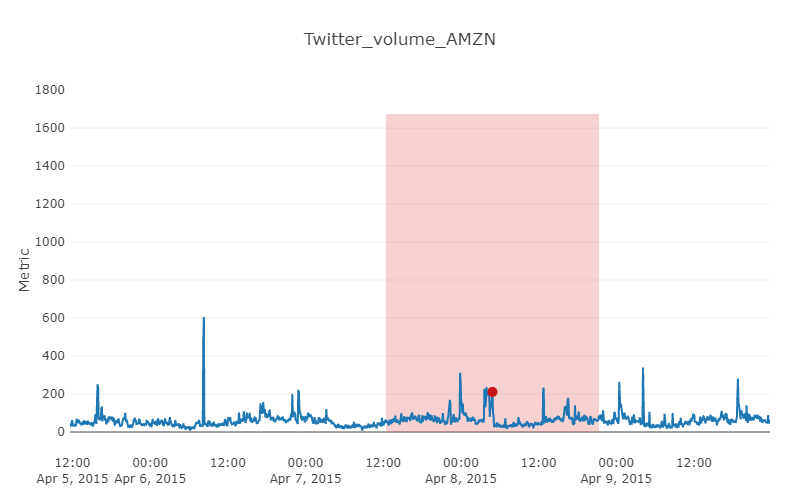
\includegraphics[width=.6\textwidth]{anomaly_windows.png}
        \caption{Example of an \defref{def:anomaly-window}. Illustration
        by the author.}\label{fig:anomaly-window}
    \end{figure}
\end{definition}
If multiple detections exist within a window, only the first detection is scored.
Additional detections within the window are ignored~\cite[cf.][]{Lavin.2015}.
Detections earlier in the window give higher positive scores than later detections.
Detections outside the anomaly window give negative scores.

Details on the calculation of the scoring function are given in \cref{app:numenta-score}
and an exemplary application is depicted in \cref{fig:anomaly-score-example}.


\paragraph{Visual Examination}
In this paragraph, an overview of the most common anomaly types within the \gls{nab}
is given. From visual observation only, the vast majority (about 30) of time
series from the dataset contain point anomalies~\cref{fig:point-anomalies-nab}.
Other more common types include contextual anomalies \cref{fig:contextual-anomalies-nab}.
Collective anomalies only appear in form of change points. A very good example
for collective anomalies however, as the one from \cref{fig:collective-anomalies-nab},
is not found within \gls{nab}.

Regarding triviality allegations from \textcite{Lavin.2015}, \(\sim 1/3\) of
point anomalies are so far from their neighborhood, that \(\mu_t + 3*\sigma_t\)
(\(\mu_t, \sigma_t\) are the moving mean and the moving standard deviation
respectively) would suffice to detect them, e.g.\ \cref{fig:point-anomalies-nab}.
This implies triviality of the dataset. However, such trivial solution would
also detect many false positives. While, from short examination, it appears possible
to solve many of the time series presented in \gls{nab} with comparatively simple
statistical operations, such a solution would probably require a unique set of such
operations for every time series. Thereby defeating the purpose of \gls{nab} of
scoring a unified algorithm that must \textit{not} be adjusted for every such
time series.

Additional plots from the dataset can be found in \cref{sect:additonal-plots-dataset}.

\begin{figure}[htp!]
    \centering
    \begin{subfigure}[t]{.49\linewidth}
        \centering
        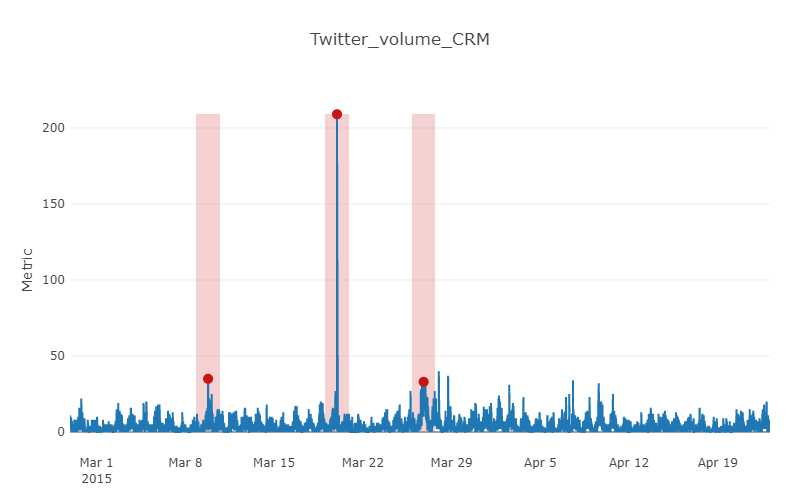
\includegraphics[width=\textwidth]{anomaly_types_examples/final/png/Twitter_volume_CRM.png}
    \end{subfigure}
    \begin{subfigure}[t]{.49\linewidth}
        \centering
        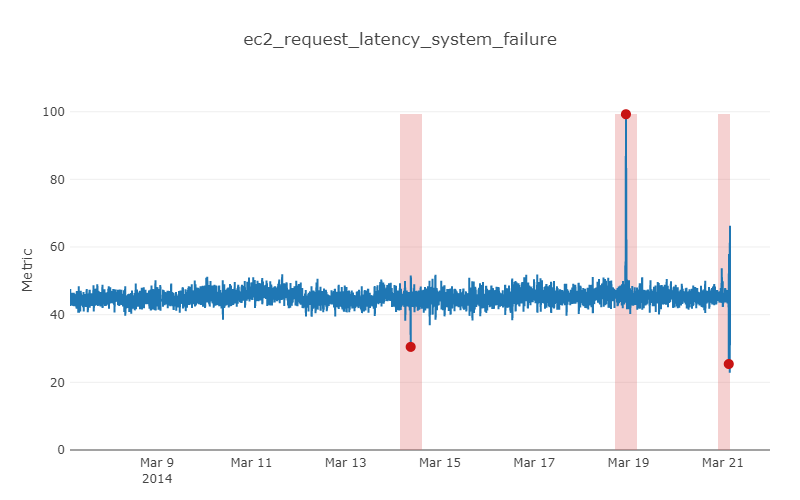
\includegraphics[width=\textwidth]{anomaly_types_examples/final/png/ec2_request_latency_system_failure.png}
    \end{subfigure}
    \caption{Two examples of Point Anomalies}\label{fig:point-anomalies-nab}
\end{figure}

\begin{figure}[htp!]
    \centering
    \begin{subfigure}[t]{.49\linewidth}
        \centering
        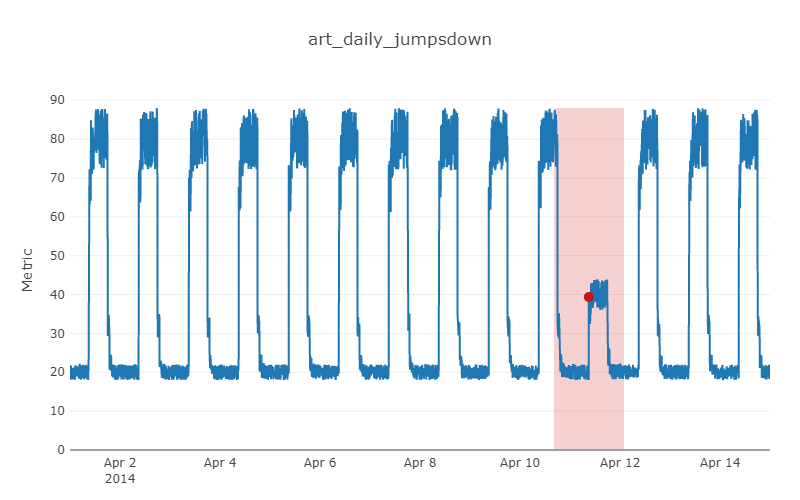
\includegraphics[width=\textwidth]{anomaly_types_examples/final/png/art_daily_jumpsdown.png}
    \end{subfigure}
    \begin{subfigure}[t]{.49\linewidth}
        \centering
        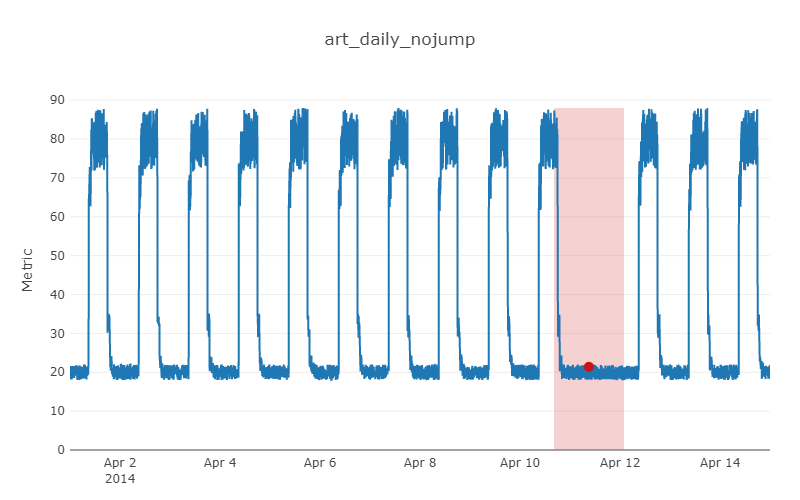
\includegraphics[width=\textwidth]{anomaly_types_examples/final/png/art_daily_nojump.png}
    \end{subfigure}
    \caption{Two examples of (artificial) cyclicity violations (contextual anomalies)}\label{fig:contextual-anomalies-nab}
\end{figure}

\begin{figure}[htp!]
    \centering
    \begin{subfigure}[t]{.49\linewidth}
        \centering
        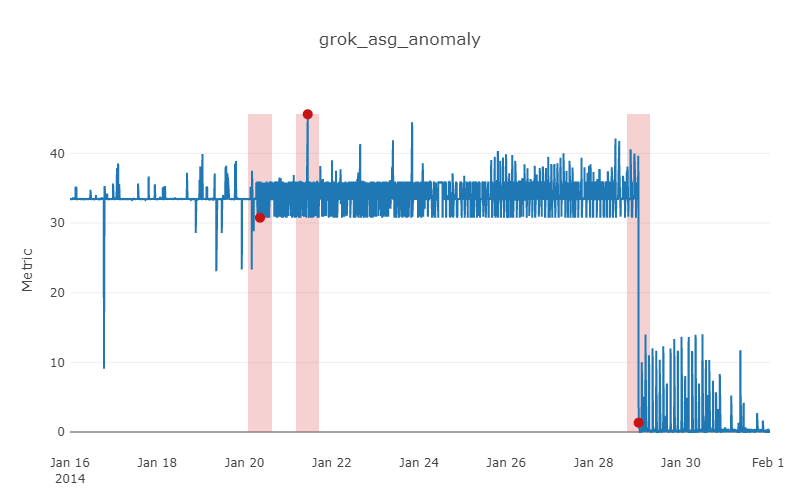
\includegraphics[width=\textwidth]{anomaly_types_examples/final/png/grok_asg_anomaly.png}
    \end{subfigure}
    \caption{An example of two change points (collective anomalies) and a point anomaly}\label{fig:collective-anomalies-nab}
\end{figure}\todo{Is clearpage still required?}
\clearpage

\subsection{Algorithm overview}
In an attempt to reduce the implementation complexity required for this paper,
the majority of algorithms has been adopted from open source libraries and
adjusted slightly for application to the \gls{nab} dataset.\footnote{Customization most notably
included the partition of time series into multiple subsets that were alternatingly
used for training and inference.} On GitHub, several repositories can be found
which curate lists of such libraries. All repositories used for this process are
listed in \cref{tab:curation-lists}.

From these repositories, all libraries that offer algorithms belonging to either
\invdefref{def:forecasting-based-algo} or \invdefref{def:boundary-based-algo}
are listed in the appendix (forecasting-based: \cref{def:forecasting-based-algo},
boundary-based: \cref{tab:ad-packages}). Both tables contain three columns:
an (almost exhaustive) list of models offered by the library, the latest
released version, and the date of the latest commit.

Then, a subset of ten libraries is chosen. Five of them with a focus on forecasting
and the remaining five with a focus on boundaries. Libraries that are found within
another library are dropped from the list (e.g.\ \(\text{Prophet, GluonTS } \in \text{ AtsPy}\)).
Finally, a set of libraries is picked by the author, whereby recently updated libraries,
libraries with sufficient documentation and libraries with a high number of
stars (measuring to an extent the appreciation of the community) are slightly
preferred. The chosen libraries are presented in \cref{tab:chosen-packages}.

From these ten libraries, a subset of algorithms is selected. The selected
forecasting-algorithms are shown in \cref{tab:chosen-forecasting-algo},
boundary-algorithms are shown in \cref{tab:chosen-boundary-algo}.

If not stated otherwise, default parameters from within the libraries are adopted.

\section{Results and Discussion}\label{sect:results-and-discussion}
\blindtext[1]

\subsection{NAB-Scores}
\blindtext[3]

\subsection{Visual Evaluation}
\blindtext[3]

\section{Conclusion}\label{sect:conclusion}
Time series from \gls{nab} are not able to answer specific questions on the
behavior of algorithms
\blindtext[1]

\subsection{Recommendations}\label{subsect:recommendations}
\blindtext[1]

\subsection{Future Work}
\blindtext[1]


%%%% Backmatter %%%%
\clearpage
\pagenumbering{roman} % Continued roman page numbering backmatter
\setcounter{page}{\value{roman-pagenumber} + 1} % set page number to counter+1
{
  \hypersetup{hidelinks}
  \printbibliography[title={Bibliography}]
}
\appendix
\section{Details on phase b.\ of forecasting-based algorithms}\label{sec:forecasting-eval}
As noted in \cref{subsect:how-are-we-retrieving-it}, the evaluation of forecasting
errors is not part of (most) available forecasting packages. Therefore, a variety
of approaches was adopted for this paper. Most trivially, a moving mean and standard
deviation were used as a dynamic threshold. Every forecasting error exceeding this
threshold was remarked as a detection (\cref{def:detection}). Both 
\begin{enumerate*}
    \item using an \gls{ocsvm} and 
    \item identifying the best fitting distribution, then performing p-tests was
    disregarded for every forecasting error
\end{enumerate*}
were disregarded for their computational complexity and subpar results.

More complex scoring methods from~\cite{Ahmad.2017,Hundman.2018} were adopted.
While the method from \textcite{Ahmad.2017} is illustrated in this section,
non-parametric thresholding from \textcite{Hundman.2018} was able to outperform
it in every application and was therefore used to produce the final results.
For details please review~\cite{Hundman.2018}.

\textcite{Ahmad.2017} suggest modelling the distribution of errors as a rolling normal
distribution with mean and standard deviation \(\mu_t, \sigma_t\) according to
\cref{eq:rolling-mean,eq:rolling-std}

\begin{align}
    \mu_t&= \frac{\sum_{i=0}^{i=W-1}s_{t-i}}{W}\label{eq:rolling-mean}\\
    \sigma_t &= \frac{\sum_{i=0}^{i=W-1}{(s_{t-i}-\mu_t)}^2}{W - 1}\label{eq:rolling-std}
\end{align}
where:
\begin{conditions}
    W &:= & Window size, set to \(W=8000\) as proposed by~\cite{Ahmad.2017}
\end{conditions}

and a short term rolling average \(\tilde{\mu}_t\) according to \cref{eq:short-rolling-mean}.

\begin{equation}
    \tilde{\mu}_t = \frac{\sum_{i=0}^{i=W'-1}s_{t-i}}{W'}\label{eq:short-rolling-mean}\\
\end{equation}
where:
\begin{conditions}
    W' &:= & Short-term window size, set to \(W'=10\) as proposed by~\cite{Ahmad.2017}
\end{conditions}

The likelihood (\cref{eq:likelihood}) is calculated using the \gls{cdf} of a normal gaussian distribution
given in \cref{eq:cdf}
as
\begin{align}
    L_t &= \text{CDF}\left(\frac{\tilde{\mu}_t - \mu_t}{\sigma_t}\right)\label{eq:likelihood}\\
    \text{CDF}(x) &= \frac{1}{2} \left(1 + \text{erf}(\frac{x-\mu}{\sqrt{2\sigma}})\right)\label{eq:cdf}
\end{align}
where:
\begin{conditions}
    \mu&= & 0\\
    \sigma&= & 1\\
    \text{erf} &:= & the gaussian error function
\end{conditions}
Finally, a detection is recorded, when \(L_t \geq \epsilon \lor L_t \leq 1 - \epsilon\).
This is a slight deviation from~\cite{Ahmad.2017}, where only an upper p-test is
performed.

\section{Calculation of the Numenta Anonamly Metric Score}\label{app:numenta-score}
The Numenta Anomaly Metric Score for a single time series is the addition of
\begin{enumerate}[a.)]
    \item the sum of scores for every \defref{def:detection} (given by \cref{eq:score-per-detection}) and 
    \item the score for missed anomaly windows (false negatives) (given by \cref{eq:score-per-fn}).
\end{enumerate}

\begin{align}
    \sigma(t)&= \left(W_{TP} - W_{FP}\right) \left(\frac{1}{1 + e^{5t}}\right) - 1\label{eq:score-per-detection}\\
    \phi(F)&= W_{FN} * \bigl|F\bigr|\label{eq:score-per-fn}\\
    \text{Score}&= \left(\sum_{t\in T}{\sigma(t)}\right) + \phi(F)\label{eq:score-final}
\end{align}
where:
\begin{conditions}
    t &:= & the relative timestamp/position of the detection within the window.\\
    W_{\left\{TP, FP, FN\right\}} &:= & the weights attributed to true and false positives and false negatives respectively.\\
    F &:= & the set of false positives (anomaly windows without any detections).\\
    T &:= & the set of time stamps associated with the detections.
\end{conditions}

The final score per time series is calculated by \cref{eq:score-final}~\cite[cf][]{Lavin.2015}.
An example of the scoring function can be seen in \cref{fig:anomaly-score-example}.

\begin{figure}[htp!]
    \centering
    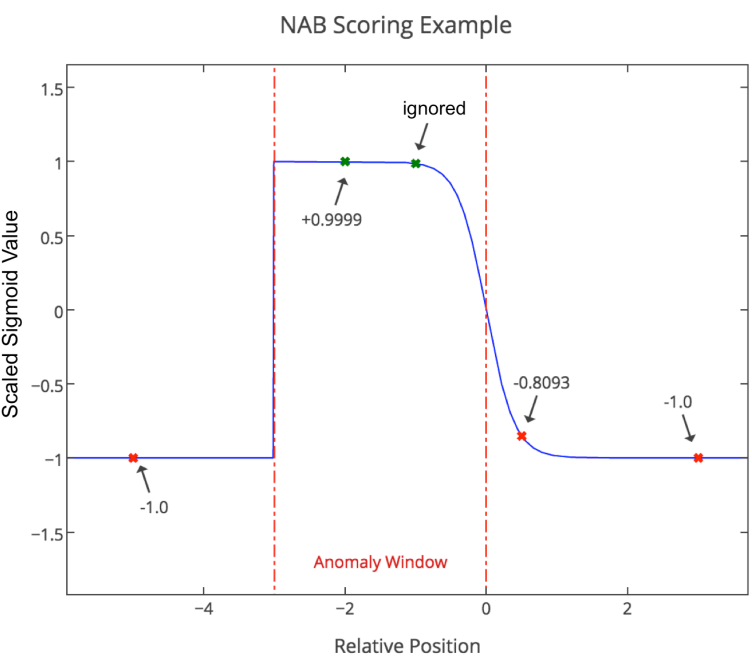
\includegraphics[width=.6\textwidth]{anomaly_scoring.png}
    \caption[Example of the anomaly scoring function]{Example application of the anomaly
    scoring function. Illustration adopted from~\cite{Lavin.2015}. The following
    text (blue) is cited from \textcite{Lavin.2015}:
    {\color{blue}
    Scoring example for a sample anomaly window, where the values
    represent the scaled sigmoid function, the second term in \cref{eq:score-per-detection}.
    The first point is an FP preceding the anomaly window (red dashed lines) and
    contributes -1.0 to the score. Within the window we see two detections, and
    only count the earliest TP for the score. There are two FPs after the window.
    The first is less detrimental because it is close to the window, and the second
    yields -1.0 because it’s too far after the window to be associated with the true
    anomaly. TNs make no score contributions. The scaled sigmoid values are
    multiplied by the relevant application profile weight, as shown in Eq.,
    the NAB score for this example would calculate as: 
    \(-1.0W_{FP} + 0.9999W_{TP} - 0.8093W_{FP} - 1.0W_{FP}\).
    With the standard application profile this would result in a total score of
    \(0.6909\).}
    }\label{fig:anomaly-score-example}
\end{figure}\clearpage

\section{Additional Plots of the Datasets}\label{sect:additonal-plots-dataset}
This section provides additional time series plots from \gls{nab}.
% Artificial Data art_daily_flatmiddle art_daily_jumpsdown art_daily_nojump art_load_balancer_spikes
\begin{figure}[htp!]
    \centering
    \begin{subfigure}[t]{.49\linewidth}
        \centering
        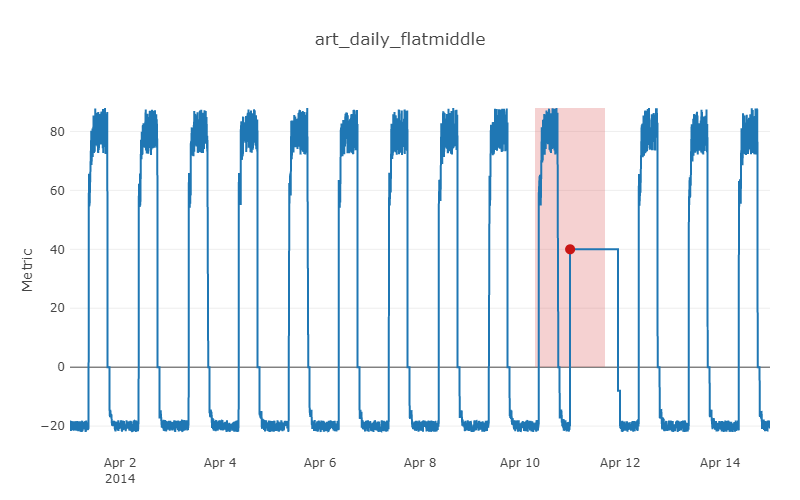
\includegraphics[width=\textwidth]{anomaly_types_examples/final/png/art_daily_flatmiddle.png}
        \subcaption{art\_daily\_flatmiddle.csv}\label{app-fig:art_daily_flatmiddle}
    \end{subfigure}
    \begin{subfigure}[t]{.49\linewidth}
        \centering
        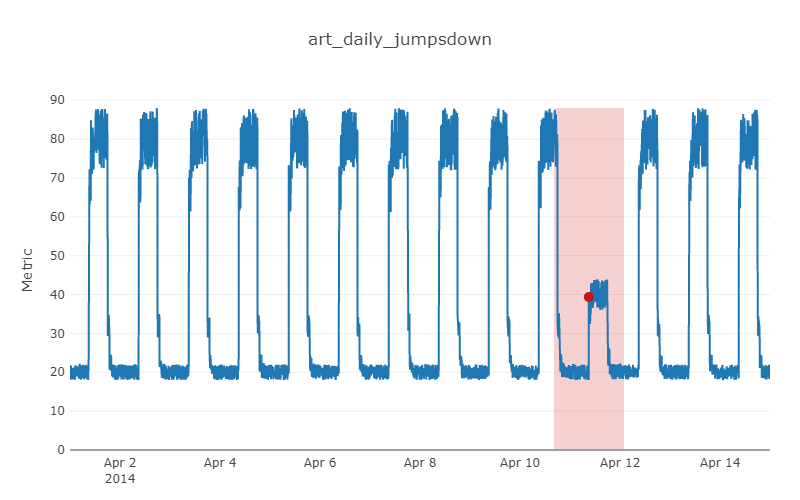
\includegraphics[width=\textwidth]{anomaly_types_examples/final/png/art_daily_jumpsdown.png}
        \subcaption{art\_daily\_jumpsdown.csv}\label{app-fig:art_daily_jumpsdown}
    \end{subfigure}
    \begin{subfigure}[t]{.49\linewidth}
        \centering
        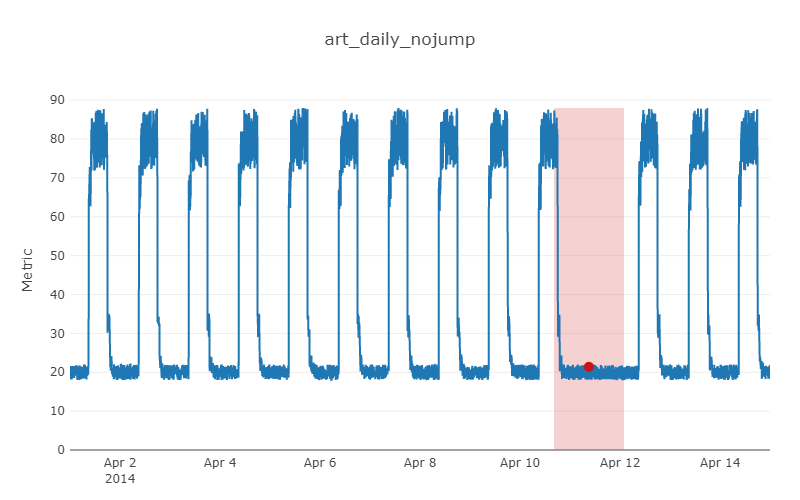
\includegraphics[width=\textwidth]{anomaly_types_examples/final/png/art_daily_nojump.png}
        \subcaption{art\_daily\_nojump.csv}\label{app-fig:art_daily_nojump}
    \end{subfigure}
    \begin{subfigure}[t]{.49\linewidth}
        \centering
        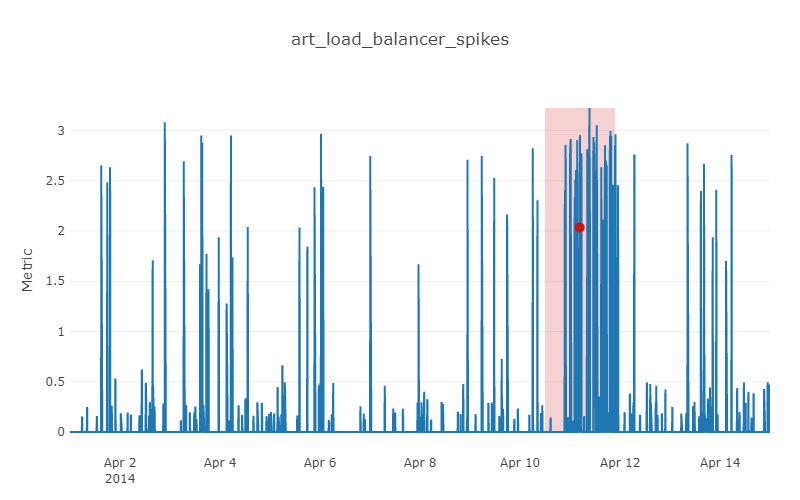
\includegraphics[width=\textwidth]{anomaly_types_examples/final/png/art_load_balancer_spikes.png}
        \subcaption{art\_load\_balancer\_spikes.csv}\label{app-fig:art_load_balancer_spikes}
    \end{subfigure}
    \caption{Artificial anomaly samples. Illustrations by the author.}\label{app-fig:artificial-anomaly-types-nab}
\end{figure}
% Mean: ec2_cpu_utilization_53ea38 grok_asg_anomaly
\begin{figure}[htp!]
    \centering
    \begin{subfigure}[t]{.49\linewidth}
        \centering
        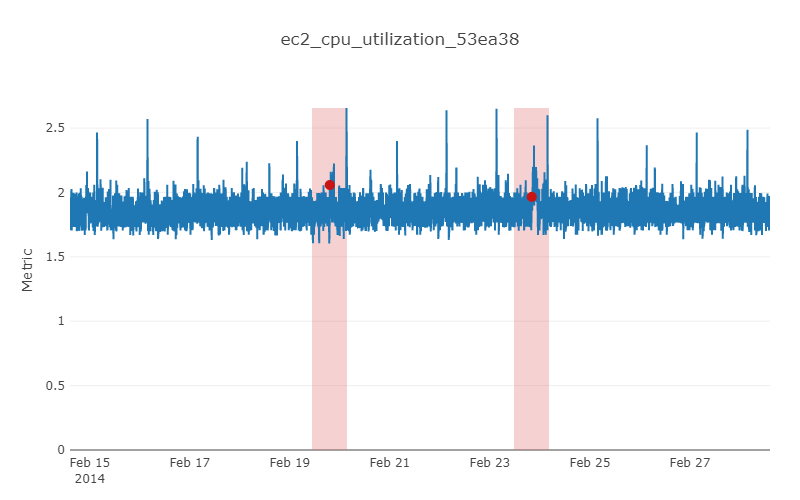
\includegraphics[width=\textwidth]{anomaly_types_examples/final/png/ec2_cpu_utilization_53ea38.png}
        \subcaption{ec2\_cpu\_utilization\_53ea38.csv}\label{app-fig:ec2_cpu_utilization_53ea38}
    \end{subfigure}
    \begin{subfigure}[t]{.49\linewidth}
        \centering
        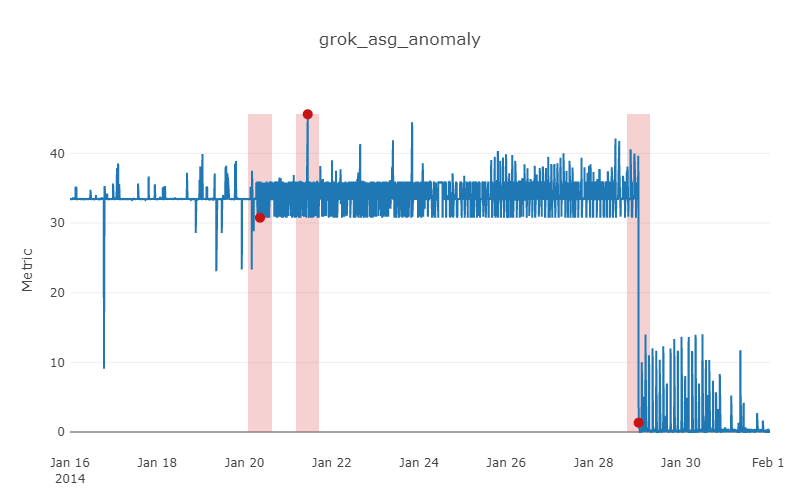
\includegraphics[width=\textwidth]{anomaly_types_examples/final/png/grok_asg_anomaly.png}
        \subcaption{grok\_asg\_anomaly.csv}\label{app-fig:grok_asg_anomaly}
    \end{subfigure}
    \caption[Contextual anomalies and change points]{(\subref{app-fig:ec2_cpu_utilization_53ea38}) 
    shows contextual anomalies, (\subref{app-fig:grok_asg_anomaly}) shows two
    change points and a point-anomaly. Illustrations by the author.}\label{fig:artificial-anomaly-types-nab}
\end{figure}
% Spikes:
% ec2_cpu_utilization_24ae8d ec2_network_in_5abac7 ec2_request_latency_system_failure elb_request_count_8c0756 Twitter_volume_CRM Twitter_volume_CVS Twitter_volume_KO ambient_temperature_system_failure
\begin{figure}[htp!]
    \centering
    \begin{subfigure}[t]{.49\linewidth}
        \centering
        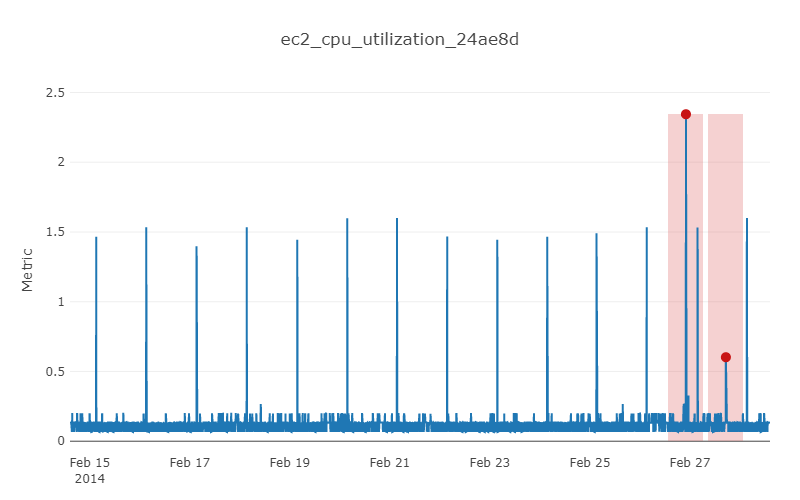
\includegraphics[width=\textwidth]{anomaly_types_examples/final/png/ec2_cpu_utilization_24ae8d.png}
        \subcaption{ec2\_cpu\_utilization\_24ae8d.csv}\label{app-fig:ec2_cpu_utilization_24ae8d}
    \end{subfigure}
    \begin{subfigure}[t]{.49\linewidth}
        \centering
        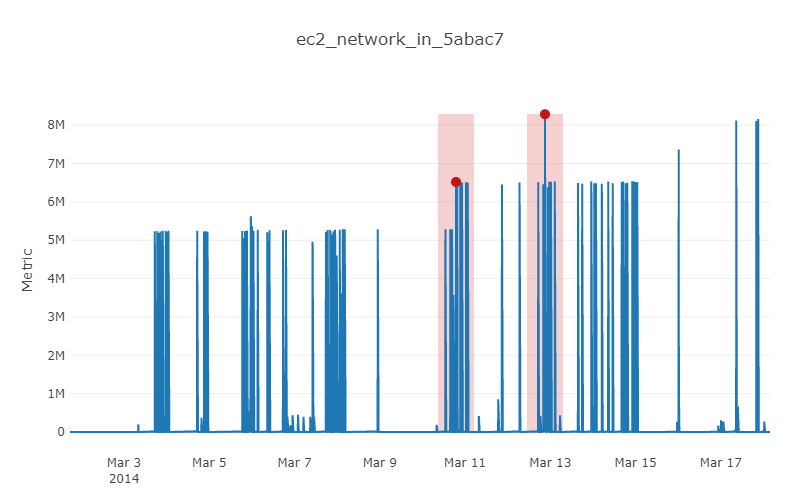
\includegraphics[width=\textwidth]{anomaly_types_examples/final/png/ec2_network_in_5abac7.png}
        \subcaption{ec2\_network\_in\_5abac7.csv}\label{app-fig:ec2_network_in_5abac7}
    \end{subfigure}
    \begin{subfigure}[t]{.49\linewidth}
        \centering
        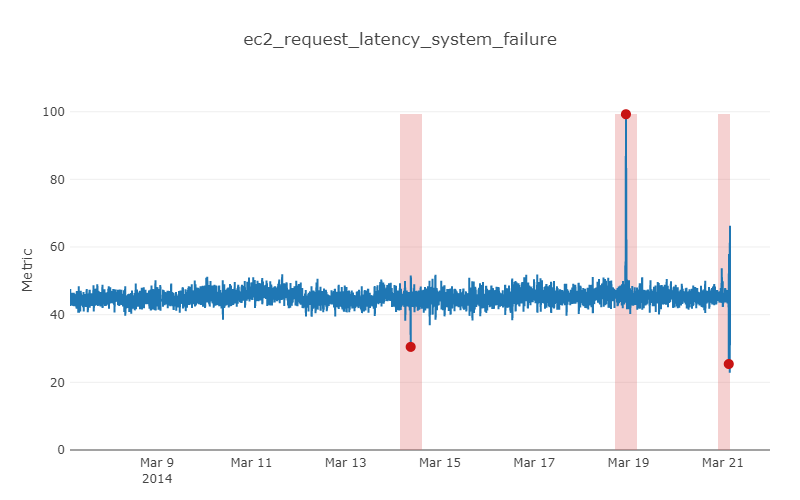
\includegraphics[width=\textwidth]{anomaly_types_examples/final/png/ec2_request_latency_system_failure.png}
        \subcaption{ec2\_request\_latency\_system\_failure.csv}\label{app-fig:ec2_request_latency_system_failure}
    \end{subfigure}
    \begin{subfigure}[t]{.49\linewidth}
        \centering
        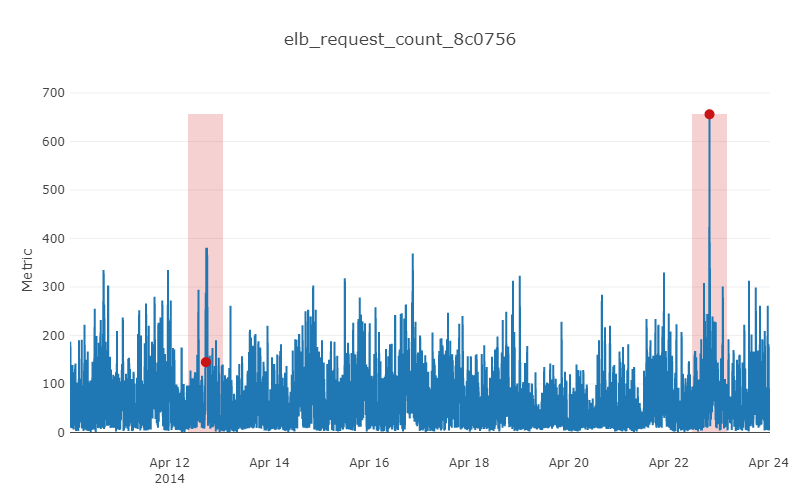
\includegraphics[width=\textwidth]{anomaly_types_examples/final/png/elb_request_count_8c0756.png}
        \subcaption{elb\_request\_count\_8c0756.csv}\label{app-fig:elb_request_count_8c0756}
    \end{subfigure}
    \begin{subfigure}[t]{.49\linewidth}
        \centering
        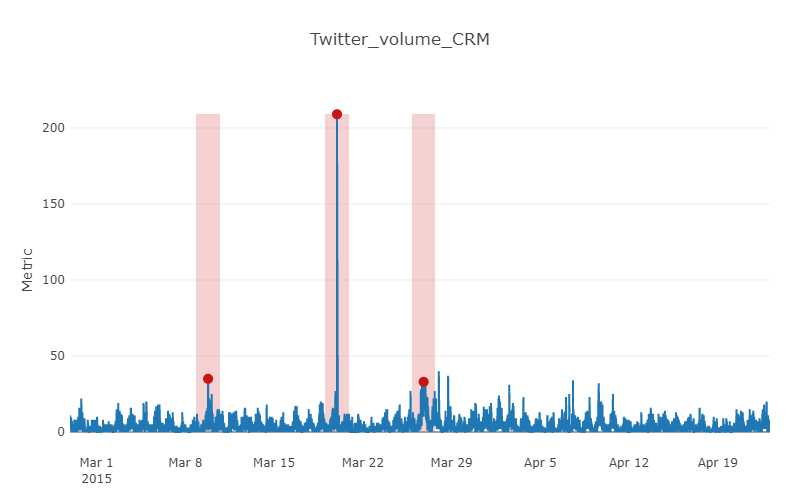
\includegraphics[width=\textwidth]{anomaly_types_examples/final/png/Twitter_volume_CRM.png}
        \subcaption{Twitter\_volume\_CRM.csv}\label{app-fig:Twitter_volume_CRM}
    \end{subfigure}
    \begin{subfigure}[t]{.49\linewidth}
        \centering
        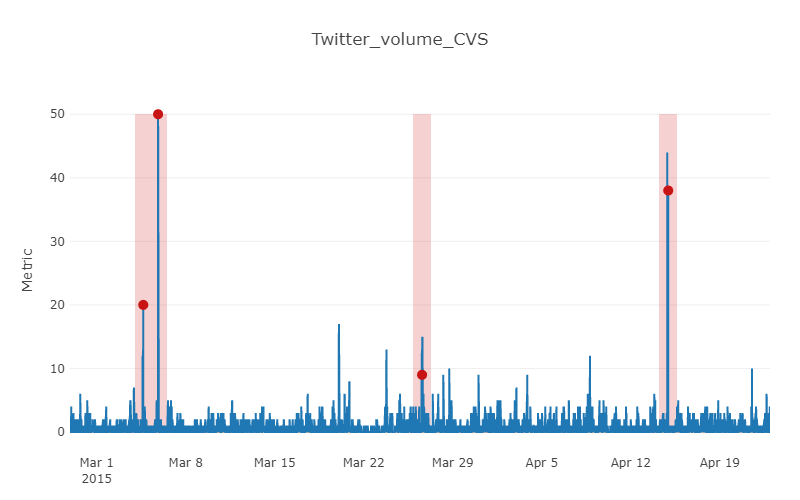
\includegraphics[width=\textwidth]{anomaly_types_examples/final/png/Twitter_volume_CVS.png}
        \subcaption{Twitter\_volume\_CVS.csv}\label{app-fig:Twitter_volume_CVS}
    \end{subfigure}
    \begin{subfigure}[t]{.49\linewidth}
        \centering
        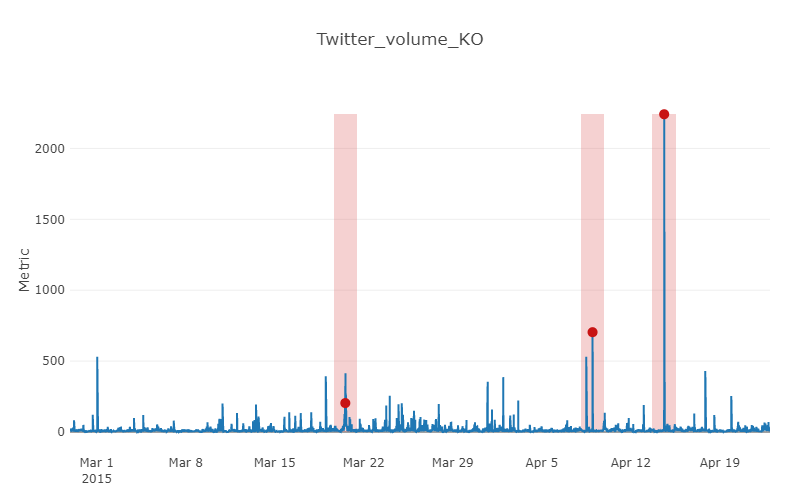
\includegraphics[width=\textwidth]{anomaly_types_examples/final/png/Twitter_volume_KO.png}
        \subcaption{Twitter\_volume\_KO.csv}\label{app-fig:Twitter_volume_KO}
    \end{subfigure}
    \begin{subfigure}[t]{.49\linewidth}
        \centering
        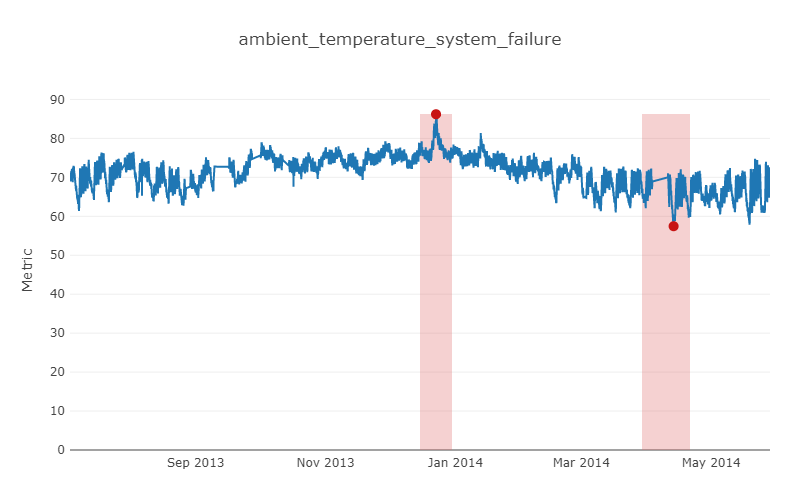
\includegraphics[width=\textwidth]{anomaly_types_examples/final/png/ambient_temperature_system_failure.png}
        \subcaption{ambient\_temperature\_system\_failure.csv}\label{app-fig:ambient_temperature_system_failure}
    \end{subfigure}
    \caption[Point Anomalies.]{Point Anomalies. All illustrations by the author.}\label{fig:spiking-types}
\end{figure}\clearpage



\section{Other Datasets}
% Table of several univariate datasets
\begin{table}[h]\centering
    \ra{1.3}
        \begin{tabular}{l}
            Dataset                                                                                                                             \\\midrule
            \href{https://github.com/numenta/NAB}{Numenta Anomaly Benchmark}                                                                    \\\addlinespace
            \href{https://www.kaggle.com/averkij/tennessee-eastman-process-simulation-dataset}{Tennessee Eastman Process Simulation Dataset}    \\\addlinespace
            \href{https://github.com/alan-turing-institute/TCPDBench}{Turing Change Point Benchmark}                                            \\\addlinespace
            \href{https://itrust.sutd.edu.sg/testbeds/secure-water-treatment-swat/}{Secure Water Treatment}                                     \\\addlinespace
            \href{https://en.wikipedia.org/wiki/Makridakis\_Competitions}{M-Competitions}                                                       \\\addlinespace
            \href{https://webscope.sandbox.yahoo.com/catalog.php?datatype=s\&did=70}{Yahoo! Webscope S5}                                        \\
        \end{tabular}
    \caption{Univariate Datasets}\label{tab:univariate-datasets}
\end{table}

% Table of several multivariate datasets
\begin{table}[h]\centering
    \ra{1.3}
        \begin{tabular}{l}
            Dataset                                                                                                                             \\\midrule
            \href{https://www.kaggle.com/anomalydetectionml/features}{Data from: Machine Learning-based Anomaly Detection in Software Systems}  \\\addlinespace
            \href{https://github.com/ricardovvargas/3w_dataset}{3W Dataset}                                                                     \\\addlinespace
            \href{https://www.kaggle.com/rkuo2000/nasa-bearing-sensor-data/notebooks}{NASA Bearing Sensor Data}                                 \\\addlinespace
            \href{https://github.com/chickenbestlover/RNN-Time-series-Anomaly-Detection}{HOT SAX Datasets}                                      \\\addlinespace
            \href{https://github.com/khundman/telemanom}{Soil Moisture Active Passive (SMAP)}                                                   \\\addlinespace
            \href{https://github.com/khundman/telemanom}{Mars Science Laboratory  (MSL)}                                                        \\\addlinespace
            \href{https://www.kaggle.com/icsdataset/hai-security-dataset}{HIL-based Augmented ICS}                                              \\
        \end{tabular}
        \caption{Multivariate-Datasets}\label{tab:multivariate-datasets}
\end{table}\clearpage


\section{Algorithm Selection}\label{sect:algorithms}
% Curation from
\begin{table}[h]\centering
    \ra{1.3}
    \begin{tabular}{l}
        Curated List                                                        \\\midrule                                                                               
        \url{https://github.com/cuge1995/awesome-time-series}               \\\addlinespace                                                                               
        \url{https://github.com/xephonhq/awesome-time-series-database}      \\\addlinespace
        \url{https://github.com/MaxBenChrist/awesome_time_series_in_python} \\\addlinespace
        \url{https://github.com/cuge1995/awesome-time-series}               \\\addlinespace
        \url{https://github.com/yzhao062/anomaly-detection-resources}       \\\addlinespace
        \url{https://github.com/rob-med/awesome-TS-anomaly-detection}       \\\addlinespace
        \url{https://www.kaggle.com/general/185462}                         \\
    \end{tabular}
    \caption{Curated lists for open source anomaly detection libraries}\label{tab:curation-lists}
\end{table}

% Libraries for forecasting
\begin{table}[h]\centering
    \ra{1.3}
    \resizebox{\textwidth}{!}{%
        \begin{tabular}{lllll}
            Library                                                                                     & Models                                                                                                                                                                                                                                                                                                                            & Version   & Latest Commit         & Stars \\\midrule
            \href{https://github.com/firmai/atspy}{AtsPy}                                               & \makecell[l]{Conglomeration of independent libraries:\\\tabitem{} Auto ARIMA\\\tabitem{} Prophet\\\tabitem{} N-Beats\\\tabitem{} Gluon-TS\\\tabitem{} and TBAT;\\ Also:\\\tabitem{} Holt Winters}                                                                                                                                              & /         & 12th Nov 2020         & 320   \\\addlinespace
            \href{https://github.com/awslabs/gluon-ts}{GluonTS}                                         & \makecell[l]{Deep Learning:\\\tabitem{} Deep Factors for Forecasting~\cite{Wang.2019}\\\tabitem{} DeepAR~\cite{Flunkert.2017}\\\tabitem{} Deep State Space~\cite{Rangapuram.2018}\\\tabitem{} Gaussian Processes\\\tabitem{} N-Beats~\cite{Oreshkin.2020}\\\tabitem{}  Transformer\\\tabitem{}  Wavenet\\Also Includes:\\\tabitem{}  Prophet}     & 0.6.4     & 7th Jan 2021          & 1.7k  \\\addlinespace
            \href{https://github.com/alkaline-ml/pmdarima}{pmdarima}                                    & SARIMAX                                                                                                                                                                                                                                                                                                                           & 1.8       & 2nd December 2020     & 790   \\\addlinespace
            \href{https://github.com/RJT1990/pyflux}{PyFlux}                                            & ARIMAX, Dynamic AR, Dynamic Linear Regression, EARCH, GAS, ARCH, GARCH\ldots                                                                                                                                                                                                                                                      & /         & 16th December 2018    & 1.8k  \\\addlinespace
            \href{https://github.com/alan-turing-institute/sktime}{sktime}                              & ARIMA, Exponential Smoothing/Holt Winters, Polynomial Thresholding                                                                                                                                                                                                                                                                & 0.5.1     & 6th Jan 2021          & 3.4k  \\\addlinespace
            \href{https://github.com/bashtage/arch}{ARCH}                                               & AR, Heterogeneous Autoregression, ARCH, GARCH, TARCH, EGARCH, \ldots                                                                                                                                                                                                                                                              & 4.15      & 7th Jan 2021          & 630   \\\addlinespace
            \href{https://github.com/LongxingTan/Time-series-prediction}{Time Series Prediction TF2}    & LSTM, GRU, Wavenet, Transformer, N-Beats, GAN                                                                                                                                                                                                                                                                                     & /         & 25th December 2020    & 292   \\\addlinespace
            \href{https://github.com/maxjcohen/transformer}{Transformers for Timer Series}              & Transformer                                                                                                                                                                                                                                                                                                                       & 0.3       & 10th December 2020    & 231   \\\addlinespace
            \href{https://github.com/facebook/prophet}{Prophet}                                         & \makecell[l]{General Additive Model\\\tabitem{} trend is fitted via a logistic or a linear model\\\tabitem{} seasonality is fitted via Fourier series\\\tabitem{} also considers holidays}                                                                                                                                              & 0.6       & 7th Jan 2021          & 12.1k \\\addlinespace
            \href{https://github.com/intive-DataScience/tbats}{TBATS}                                   & Automated BATS/TBATS fitting                                                                                                                                                                                                                                                                                                      & 1.1       & 27th July 2020        & 84    \\\addlinespace
            \href{https://github.com/philipperemy/n-beats}{N-Beats}                                     & Res- and fully connected layer                                                                                                                                                                                                                                                                                                    & /         & 30th April 2020       & 326   \\
        \end{tabular}
    }
    \caption{Forecasting-Focused Libraries, accessed last: 8th Jan 2021}\label{tab:forecasting-packages}
\end{table}

% Libraries for anomaly detection
\begin{table}[h]\centering
    \ra{1.3}
    \resizebox{\textwidth}{!}{%
        \begin{tabular}{lllll}
            Library                                                                                                 & Models    & Version   & Latest Commit     & Stars \\\midrule
            \href{https://github.com/arundo/adtk}{Anomaly Detection Toolkit (ADTK)}                                 & \makecell[l]{Statistical Models:\\\tabitem{} AR\\\tabitem{} Seasonal Pattern/Decomposition\\\tabitem{} Generalized ESD-Test\\\tabitem{} Difference in Mean\\\tabitem{} Difference in QR/IQR\\\tabitem{} Difference in Volatility; \\\\ML:\\\tabitem{} Clustering}                                                                                                                                                                           & 0.6.2     & 17th April 2020   & 582   \\\addlinespace
            \href{https://github.com/smirmik/CAD}{Contextual Anomaly Detector}                                      & No Documentation. Winner of NAB 2016                                                                                                                                                                                                                                                                                                                                                                                          & /         & 10th August 2016  & 63    \\\addlinespace
            \href{https://github.com/MentatInnovations/datastream.io}{datastream.io}                                & \makecell[l]{Focused on integration into ELK-stack;\\ Gaussian-Distribution and Difference in Percentile}                                                                                                                                                                                                                                                                                                                     & /         & 20th Feb 2018     & 804   \\\addlinespace 
            \href{https://github.com/NetManAIOps/donut}{DONUT}                                                      & Variational Auto-Encoder~\cite{Xu.2018}                                                                                                                                                                                                                                                                                                                                                                                       & /         & 6th March         & 298   \\\addlinespace 
            \href{https://github.com/hastic}{hastic}                                                                & \makecell[l]{Focused on Grafana.\\Thresholding on seasonality adjusted and exponentially smoothed data.}                                                                                                                                                                                                                                                                                                                      & /         & 26th Dec 2020     & 274   \\\addlinespace 
            \href{https://github.com/linkedin/luminol}{luminol}                                                     & Bitmap-Transformation~\cite{Wei.2005}, Single Exponential Smoothing;                                                                                                                                                                                                                                                                                                                                                          & 0.4       & 9th Jan 2018      & 861   \\\addlinespace 
            \href{https://github.com/datamllab/pyodds}{PyODDS} / \href{https://github.com/yzhao062/pyod}{PyOD}      & \makecell[l]{Statistical Models:\\\tabitem{} Local Outlier Factor\\\tabitem{} Clustering Based Local Outlier Factor\\\tabitem{} Histogram-Based Outlier Score\\\tabitem{} Isolation Forest\\\tabitem{} kNN\\\tabitem{} One-Class SVM\\\tabitem{} PCA\\\tabitem{} Robust Covariance\\\tabitem{} Subspace Outlier Detection\\\tabitem{} Luminol\\ Deep Learning:\\\tabitem{} LSTMAD\cite{Malhotra.2015}\\\tabitem{} DAGMM~\cite{Zong.2018}}             & /         & 8th May 2020      & 132   \\\addlinespace 
            \href{https://github.com/kLabUM/rrcf}{rrcf}                                                             & Robust Random Cut Forest~\cite{Guha.2016}                                                                                                                                                                                                                                                                                                                                                                                     & 0.4.3     & 10th June 2020    & 271   \\\addlinespace 
            \href{https://github.com/chickenbestlover/RNN-Time-series-Anomaly-Detection}{rnn ts anomaly detection}  & LSTM, GRU, SRU                                                                                                                                                                                                                                                                                                                                                                                                                & /         & 21st Oct 2020     & 684   \\\addlinespace 
            \href{https://github.com/datamllab/tods}{TODS: Time-series Outlier Detection System}                    & DeepLog~\cite{Du.2017}, Telemanom Matrix Profile, PyOD algorithms                                                                                                                                                                                                                                                                                                                                                             & /         & 5th Jan 2021      & 258   \\\addlinespace
            \href{https://github.com/earthgecko/skyline}{Skyline}                                                   & Ensemble of statistical tests like Kolmogorov-Smirnov, Grubbs, deviation from median\ldots                                                                                                                                                                                                                                                                                                                                    & 2.0       & 22nd Dec 2020     & 284   \\\addlinespace
            \href{https://github.com/tsurubee/banpei}{Banpei}                                                       & Hotelling's theory~\cite{Hotelling.1990} and Singular Spectrum Transformation                                                                                                                                                                                                                                                                                                                                                 & /         & 21st Sept 2020    & 222   \\\addlinespace
            \href{https://github.com/htm-community/htm.core}{NuPIC}                                                 & Numenta HTM                                                                                                                                                                                                                                                                                                                                                                                                                   & /         & 23 Oct 2019       & 6.2k   \\\addlinespace
            \href{https://github.com/matrix-profile-foundation/matrixprofile}{MPF}                                  & Matrix Profile                                                                                                                                                                                                                                                                                                                                                                                                                & /         & 26th Dec 2020     & 121    \\
        \end{tabular}
    }
    \caption{Boundary Focused Detection Libraries, accessed last: 8th Jan 2021}\label{tab:boundary-packages}
\end{table}

% Chosen Library Anomaly Detection & Forecasting
\begin{table}[h]\centering
    \ra{1.3}
        \begin{tabular}{l}
            Boundary-Libraries \\\midrule
            \href{https://github.com/datamllab/pyodds}{PyODDS} / \href{https://github.com/yzhao062/pyod}{PyOD}      \\\addlinespace
            \href{https://github.com/kLabUM/rrcf}{rrcf}                                                             \\\addlinespace
            \href{https://github.com/earthgecko/skyline}{Skyline}                                                   \\\addlinespace
            \href{https://github.com/htm-community/htm.core}{NuPIC}                                                 \\\addlinespace\addlinespace
            Forecasting-Libraries \\\midrule
            \href{https://github.com/awslabs/gluon-ts}{GluonTS}                                                     \\\addlinespace
            \href{https://github.com/firmai/atspy}{AtsPy}                                                           \\\addlinespace
            \href{https://github.com/RJT1990/pyflux}{PyFlux}                                                        \\\addlinespace
            \href{https://github.com/alan-turing-institute/sktime}{sktime}                                          \\\addlinespace
        \end{tabular}
    \caption{Chosen Libraries}\label{tab:chosen-packages}
\end{table}

% Chosen Forecasting Algo
\begin{table}[h]\centering
    \ra{1.3}
        \begin{tabular}{ll}
            Forecasting Algorithm                                       & Package/Implementation    \\\midrule         
            Prophet~\cite{Taylor.2017}                                  & \href{https://github.com/firmai/atspy}{AtsPy}             \\\addlinespace
            Auto ARIMA~\cite{Smith.2017}                                & \href{https://github.com/alkaline-ml/pmdarima}{pmdarima}  \\\addlinespace
            ARIMA~\cite[Hyperparameters adopted from][]{Braei.2020}     & \href{https://github.com/alkaline-ml/pmdarima}{pmdarima}  \\\addlinespace
            Holt-Winters~\cite{Winters.1960}                            & \href{https://github.com/firmai/atspy}{AtsPy}             \\\addlinespace
            N-BEATS~\cite{Oreshkin.2020}                                & Implementation by the author                              \\\addlinespace
            TBAT/S                                                      & \href{https://github.com/firmai/atspy}{AtsPy}             \\\addlinespace
            DeepAnT~\cite{Munir.2019}                                   & Implementation by the author                              \\
        \end{tabular}
    \caption{Chosen Forecasting Algorithms}\label{tab:chosen-forecasting-algo}
\end{table}

% Chosen Boundary Algo
\begin{table}[h]\centering
    \ra{1.3}
        \begin{tabular}{ll}
            Boundary Algorithm                                  & Package/Implementation   \\\midrule                                                                               
            \gls{lof}~\cite{Breunig.2000}                       & \href{https://github.com/datamllab/pyodds}{PyODDS}                            \\\addlinespace
            \gls{ae}~\cite[499\psqq]{Goodfellow.2016}        & \href{https://github.com/datamllab/pyodds}{PyODDS}                            \\\addlinespace
            \gls{cblof}~\cite{He.2003}                          & \href{https://github.com/datamllab/pyodds}{PyODDS}                            \\\addlinespace
            \gls{dagmm}\cite{Zong.2018}                         & \href{https://github.com/datamllab/pyodds}{PyODDS}                            \\\addlinespace
            \gls{knn}~\cite[16\psqq]{Murphy.2012}               & \href{https://github.com/datamllab/pyodds}{PyODDS}                            \\\addlinespace
            Skyline                                             & \href{https://github.com/earthgecko/skyline}{Skyline}                         \\\addlinespace
            \gls{ocsvm}~\cite{Schölkopf.1999,Tax.2004}          & \href{https://github.com/datamllab/pyodds}{PyODDS}                            \\\addlinespace
            Robust Random Cut Forest~\cite{Bartos.2019}         & \href{https://github.com/kLabUM/rrcf}{rrcf}                                   \\\addlinespace
            LSTM-AD~\cite{Malhotra.2015}                        & \href{https://github.com/datamllab/pyodds}{PyODDS}                            \\\addlinespace
            LSTM-ED~\cite{Malhotra.2016}                        & \href{https://github.com/datamllab/pyodds}{PyODDS}                            \\\addlinespace
            Numenta Threshold Detector~\cite{Ahmad.2017}        & Implementation by the author / \href{https://github.com/numenta/nupic}{NuPIC} \\\addlinespace
            Numenta \gls{htm}~\cite{Ahmad.2017}                 & \href{https://github.com/htm-community/htm.core}{Community-HTM}               \\
        \end{tabular}
    \caption{Chosen Boundary Algorithms}\label{tab:chosen-boundary-algo}
\end{table}
\clearpage

\section{Illustrations from Forecasting Algorithms}

\begin{figure}[htp!]
    \begin{subfigure}[b]{\linewidth}
        \centering
        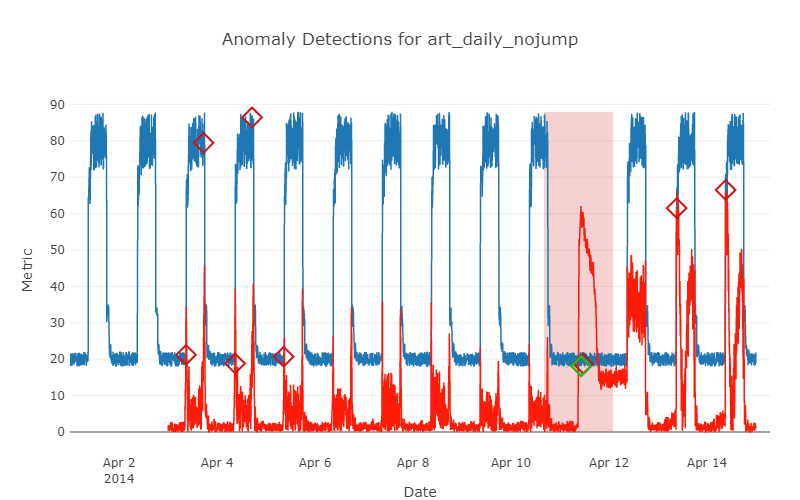
\includegraphics[width=.7\textwidth]{evaluation/deepant/cyclicity.png}
        \subcaption{Example detection of a cyclicity violation. True positives
        are displayed as green- and false positives as red diamonds. The red line
        shows error-terms from DeepAnT, the blue line shows the original time series.}\label{fig:deepant-cyclicity}
    \end{subfigure}
    \\
    \begin{subfigure}[b]{\linewidth}
        \centering
        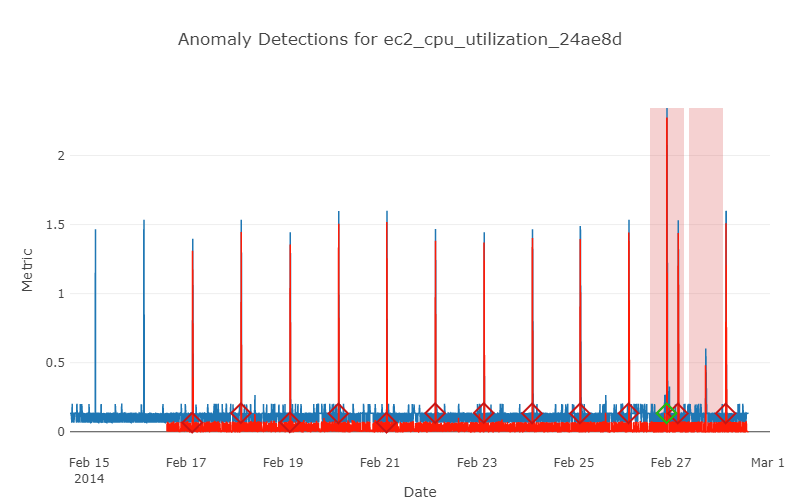
\includegraphics[width=.7\textwidth]{evaluation/deepant/resembles_original2.png}
        \subcaption{A result from DeepAnT from a time series with regular spikes.
        The error-terms (red) closely resemble the original values (blue --- 
        mostly hidden underneath the red error-terms).}\label{fig:deepant-resemble}
    \end{subfigure}
\end{figure}
\begin{figure}[htp!]
    \ContinuedFloat{}
    \begin{subfigure}[b]{\linewidth}
        \centering
        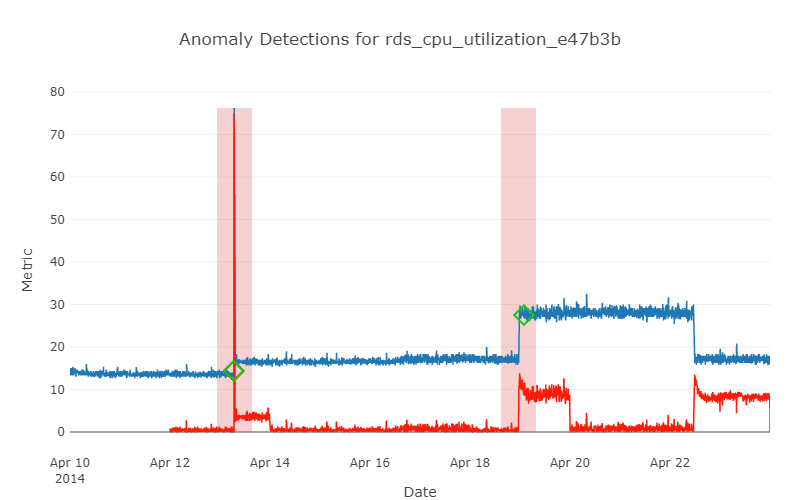
\includegraphics[width=.7\textwidth]{evaluation/deepant/changepoint_response.png}
        \subcaption{DeepAnTs response to multiple changepoints. First, predictions
        occur mean shifted. However, DeepAnT quickly adapts to the new behavior.}\label{fig:deepant-changepoint}
    \end{subfigure}
    \caption[Examples from DeepAnT.]{Examples from DeepAnT. Illustrations by the author.}\label{fig:deepant-output}
\end{figure}

\begin{figure}[htp!]
    \begin{subfigure}[b]{\linewidth}
        \centering
        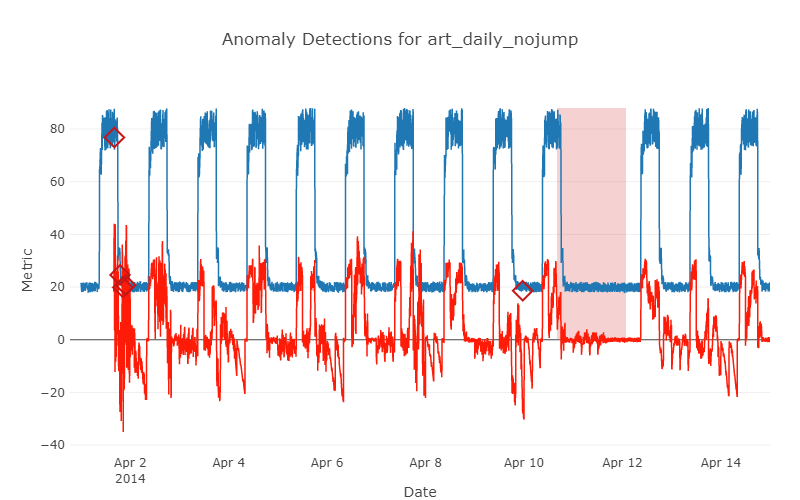
\includegraphics[width=.7\textwidth]{evaluation/nbeats/noisy2.png}
        \subcaption{An example of N-BEATS' lack of sensitivity to long-term cyclicity}\label{fig:nbeats-cyclicity}
    \end{subfigure}
    \\
    \begin{subfigure}[b]{\linewidth}
        \centering
        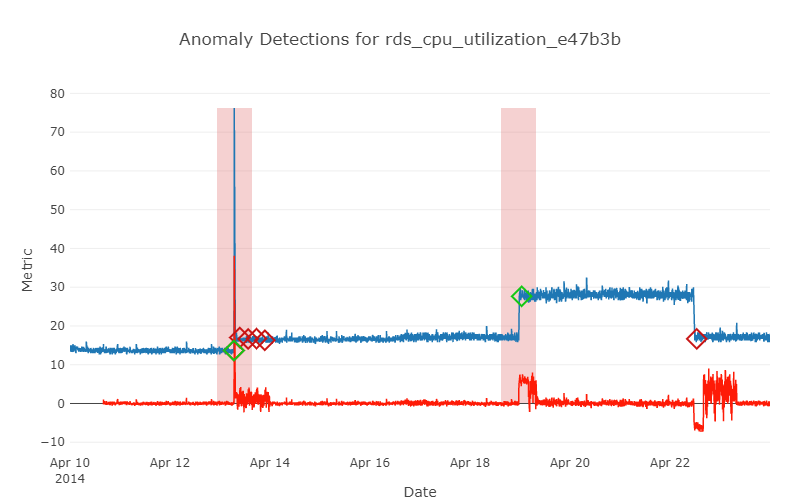
\includegraphics[width=.7\textwidth]{evaluation/nbeats/changepoints.png}
        \subcaption{Like DeepAnT, output from N-BEATS often resembles the original
        time series.}\label{fig:nbeats-resembles}
    \end{subfigure}
    \\
    \begin{subfigure}[b]{\linewidth}
        \centering
        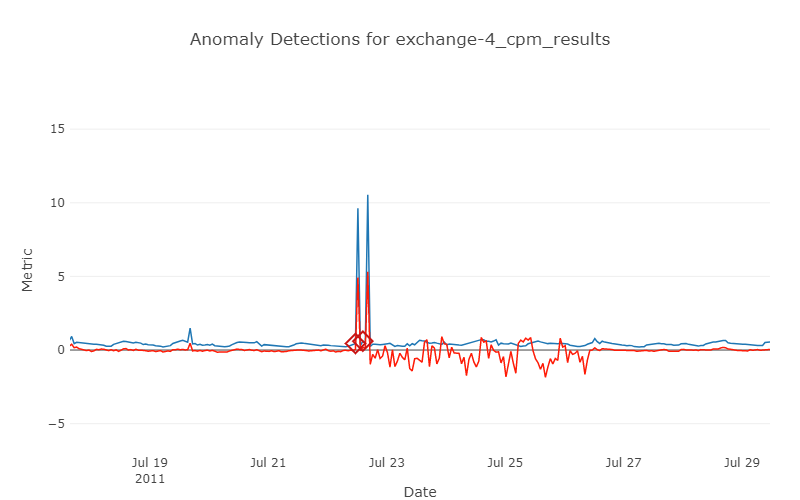
\includegraphics[width=.7\textwidth]{evaluation/nbeats/lasting_impact.png}
        \subcaption{Example of a value spike (Jul 23) that decreases prediction
        accuracy for almost four consecutive day.}\label{fig:nbeats-spike-impact}
    \end{subfigure}
    \caption[Examples from N-BEATS.]{Examples from N-BEATS\@. Illustrations by the author.}\label{fig:nbeats-output}
\end{figure}

\begin{figure}[htp!]
    \begin{subfigure}[b]{\linewidth}
        \centering
        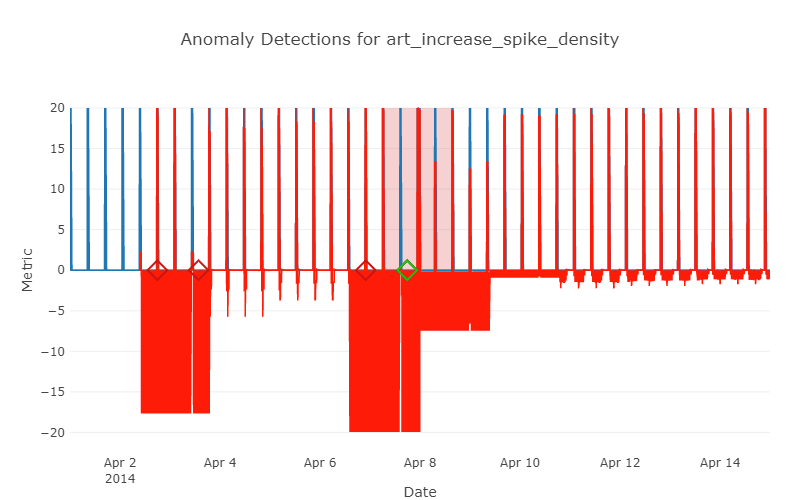
\includegraphics[width=.7\textwidth]{evaluation/hw/broken.png}
        \subcaption{An example of computational instability from Holt-Winters.}\label{fig:hw-broken}
    \end{subfigure}
    \\
    \begin{subfigure}[b]{\linewidth}
        \centering
        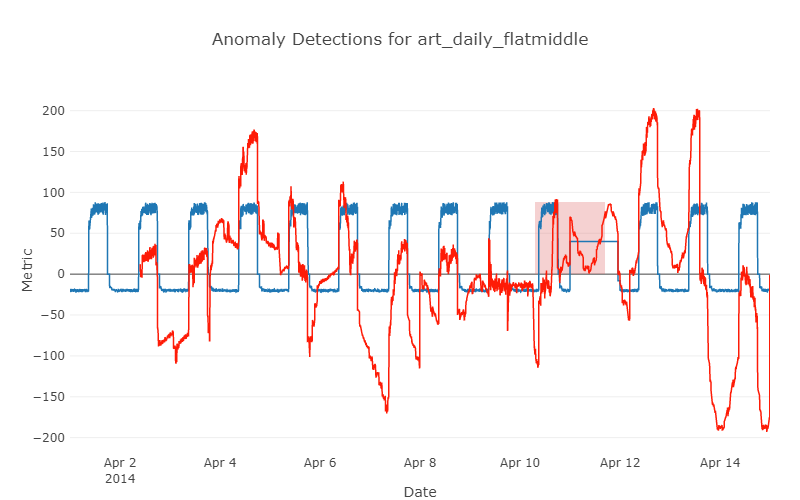
\includegraphics[width=.7\textwidth]{evaluation/hw/broken_trend.png}
        \subcaption{An example of inferred trends from Holt-Winters that are not
        found within the data.}\label{fig:hw-trend-instability}
    \end{subfigure}
    \\
    \begin{subfigure}[b]{\linewidth}
        \centering
        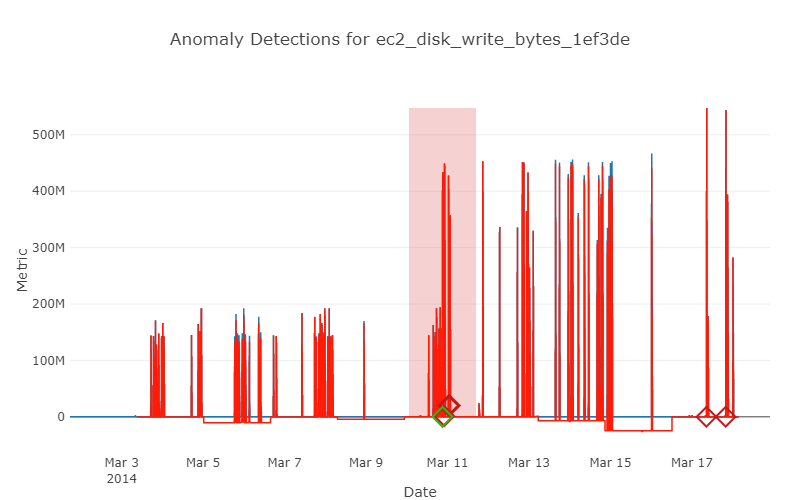
\includegraphics[width=.7\textwidth]{evaluation/hw/unstable3.png}
        \subcaption{A more ordinary example from Holt-Winters.}\label{fig:hw-ordinary}
    \end{subfigure}
    \caption[Examples from Holt-Winters.]{Examples from Holt-Winters. Illustrations by the author.}\label{fig:hw-output}
\end{figure}

\begin{figure}[htp!]
    \begin{subfigure}[b]{\linewidth}
        \centering
        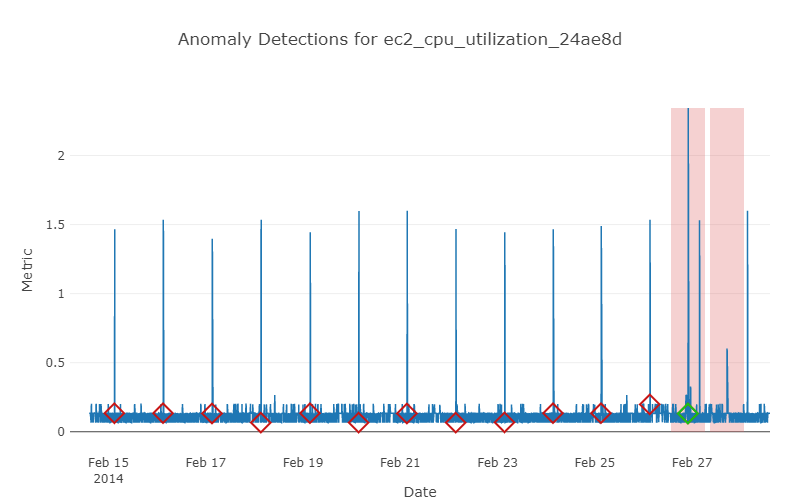
\includegraphics[width=.7\textwidth]{evaluation/arima_khundman/high_fp3.png}
        \subcaption{High false positives rate on time series with many spikes.}\label{fig:arima-fp}
    \end{subfigure}%
    \\
    \begin{subfigure}[b]{\linewidth}
        \centering
        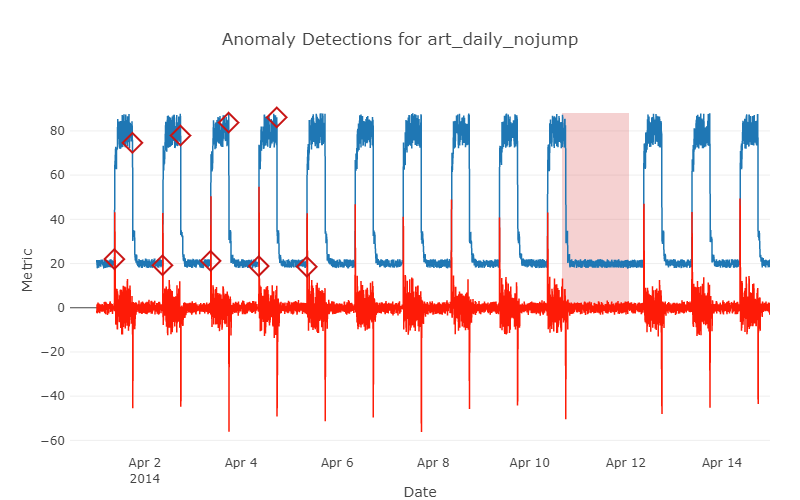
\includegraphics[width=.7\textwidth]{evaluation/arima_khundman/cyclicity2.png}
        \subcaption{ARIMA is unable to adopt long-term cyclicity.}\label{fig:arima-cyclicity}
    \end{subfigure}
    \\
    \begin{subfigure}[b]{\linewidth}
        \centering
        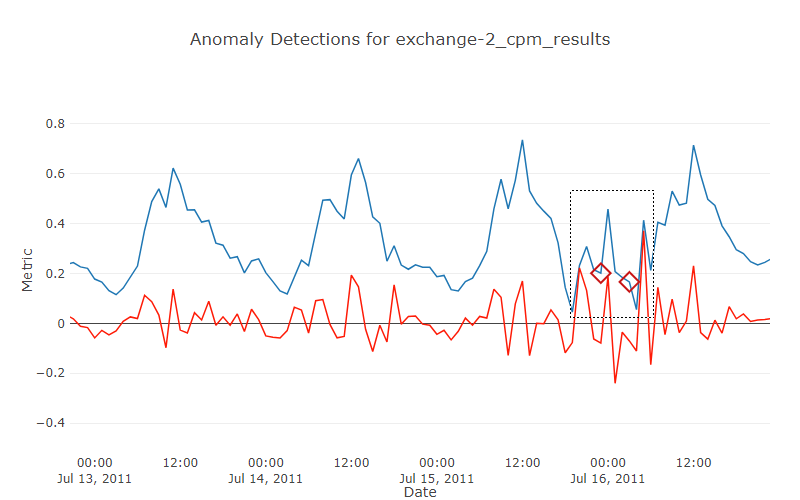
\includegraphics[width=.7\textwidth]{evaluation/arima_khundman/subtle_irregularities_box.png}
        \subcaption{Time series values are colored blue, while error-terms from ARIMA
        are red. The pattern (dotted box) from the time series deviates from previous
        time steps.}\label{fig:arima-subtle}
    \end{subfigure}
\end{figure}
\begin{figure}[htp!]
    \ContinuedFloat{}
    \begin{subfigure}[b]{\linewidth}
        \centering
        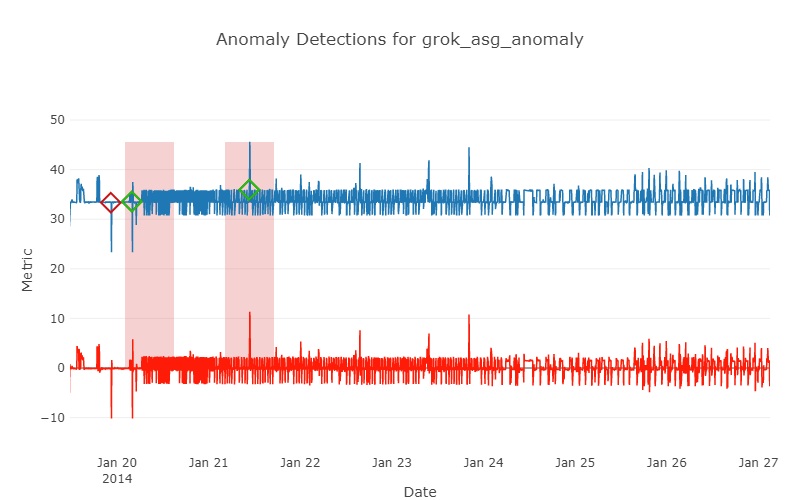
\includegraphics[width=.7\textwidth]{evaluation/arima_khundman/resembles_output3.png}
        \subcaption{On more chaotic time series, output from ARIMA closely
        resembles the original time series.}\label{fig:arima-resembles}
    \end{subfigure}
    \caption[Examples from Auto-ARIMA.]{Examples from Auto-ARIMA\@. Illustrations by the author.}\label{fig:arima-output}
\end{figure}

\begin{figure}[htp!]
    \begin{subfigure}[b]{\linewidth}
        \centering
        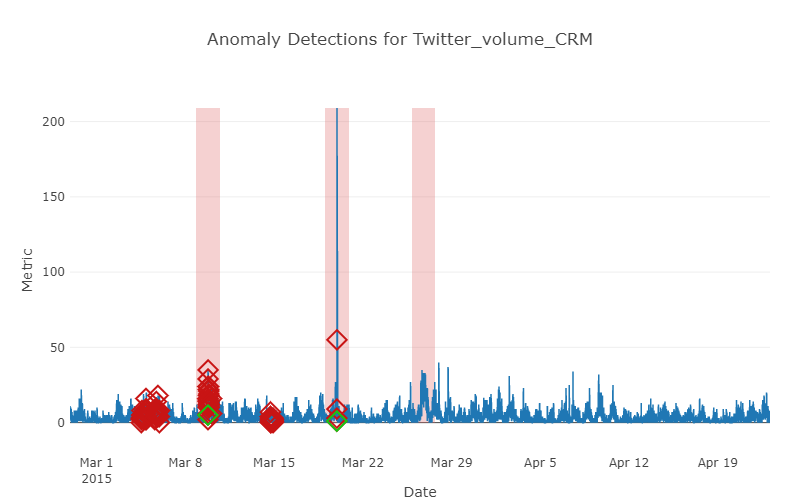
\includegraphics[width=.7\textwidth]{evaluation/prophet/high_fp5.png}
        \subcaption{57 false positives on a single time series.}\label{fig:prophet-fp}
    \end{subfigure}%
    \\
    \begin{subfigure}[b]{\linewidth}
        \centering
        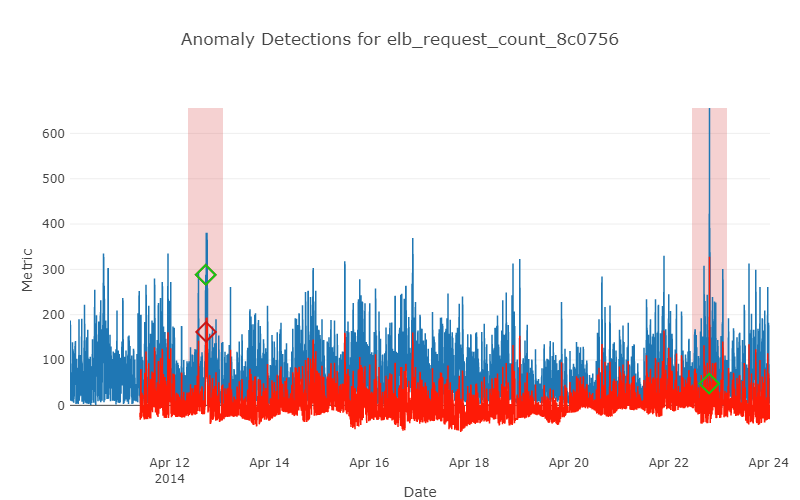
\includegraphics[width=.7\textwidth]{evaluation/prophet/noisy_low_fp.png}
        \subcaption{Prophet often assumed seasonality within the data, producing
        a curvy output.}\label{fig:prophet-curvy}
    \end{subfigure}
    \\
    \begin{subfigure}[b]{\linewidth}
        \centering
        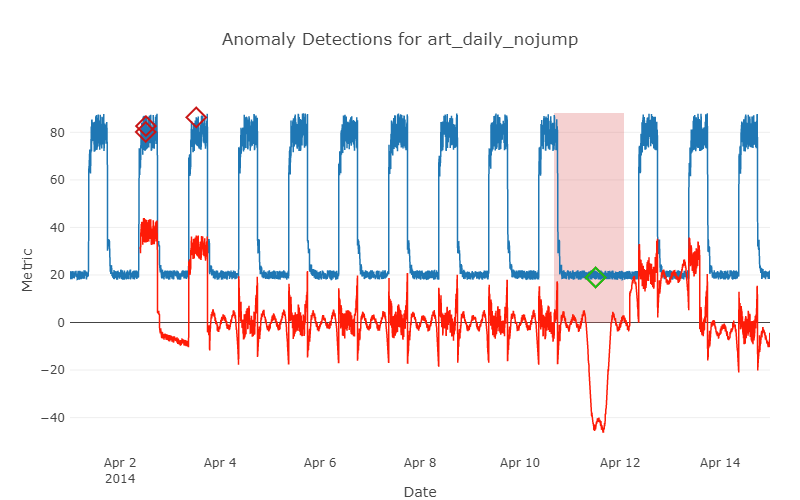
\includegraphics[width=.7\textwidth]{evaluation/prophet/cyclicity3.png}
        \subcaption{Successful adaptation to the cyclicity of a simple time series.}\label{fig:prophet-cyclicity}
    \end{subfigure}
\caption[Examples from Prophet.]{Examples from Prophet. Illustrations by the author.}\label{fig:prophet-output}
\end{figure}
\clearpage

\section{Illustrations from Boundary Algorithms}

\begin{figure}[htp!]
    \begin{subfigure}[b]{\linewidth}
        \centering
        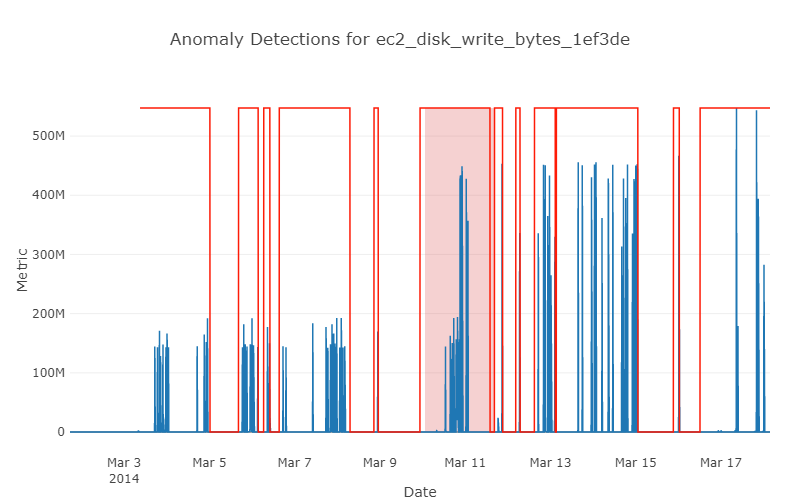
\includegraphics[width=.7\textwidth]{evaluation/ocsvm/noisy1.png}
        \subcaption{Output from \gls{ocsvm} seems to lay \textit{boxes} around
        observations with value \(> 0\). Useless output for the task of anomaly
        detection.}
    \end{subfigure}%
    \\
    \begin{subfigure}[b]{\linewidth}
        \centering
        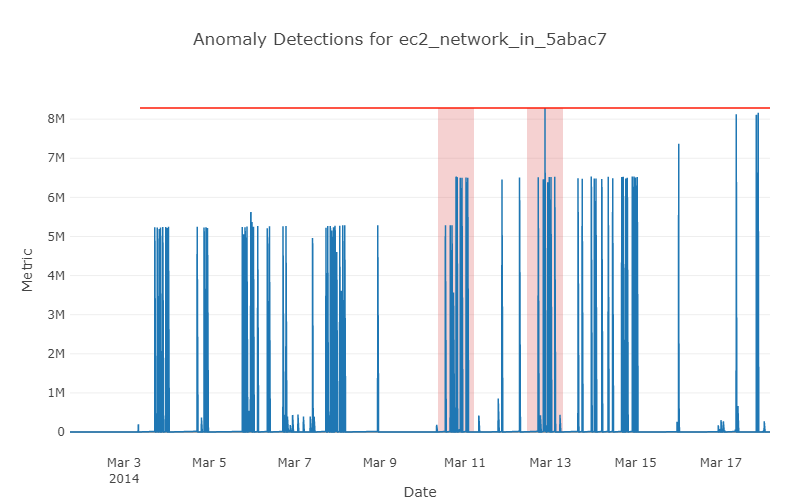
\includegraphics[width=.7\textwidth]{evaluation/ocsvm/noisy2.png}
        \subcaption{In this example, \gls{ocsvm} claims every that every 
        observation is anomalous.}
    \end{subfigure}
    \caption[Unusable outputs from \gls{ocsvm}.]{Unusable outputs from \gls{ocsvm}. Blue lines represent observations
    from the time series. Red lines represent the output from \gls{ocsvm}.
    Illustration by the author.}\label{fig:ocsvm-output}
\end{figure}

\begin{figure}[htp!]
    \begin{subfigure}[b]{\linewidth}
        \centering
        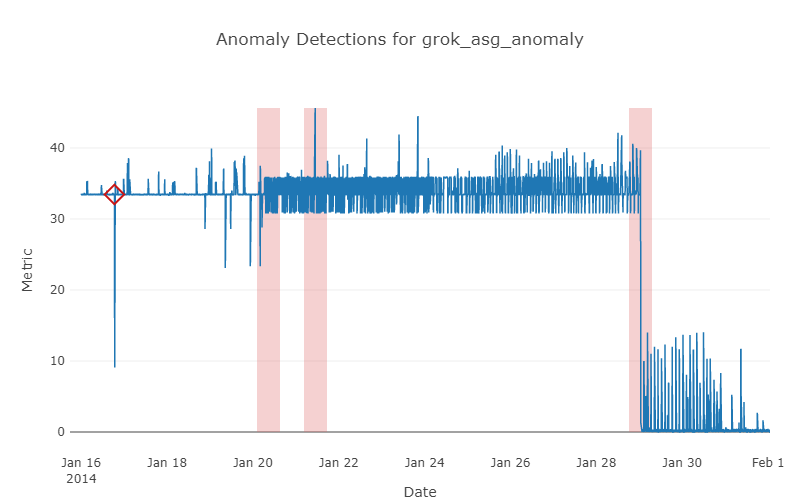
\includegraphics[width=.7\textwidth]{evaluation/lof/no_detection.png}
        \subcaption{Output from \gls{lof}, where no detections are produced on
        a seemingly simple example. Anomalous time windows are marked red.}
    \end{subfigure}%
    \\
    \begin{subfigure}[b]{\linewidth}
        \centering
        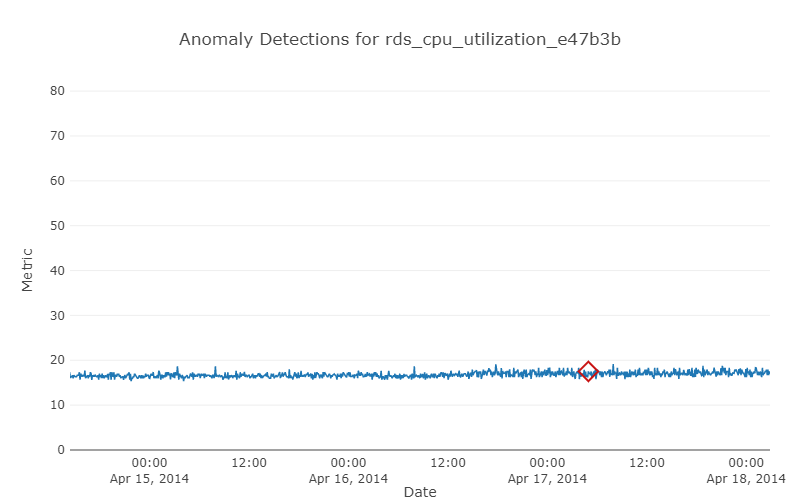
\includegraphics[width=.7\textwidth]{evaluation/lof/unreasonable_detection2.png}
        \subcaption{Example of an unreasonable detection by \gls{lof}.}
    \end{subfigure}
\end{figure}

\begin{figure}[htp!]
    \ContinuedFloat{}
    \begin{subfigure}[b]{\linewidth}
        \centering
        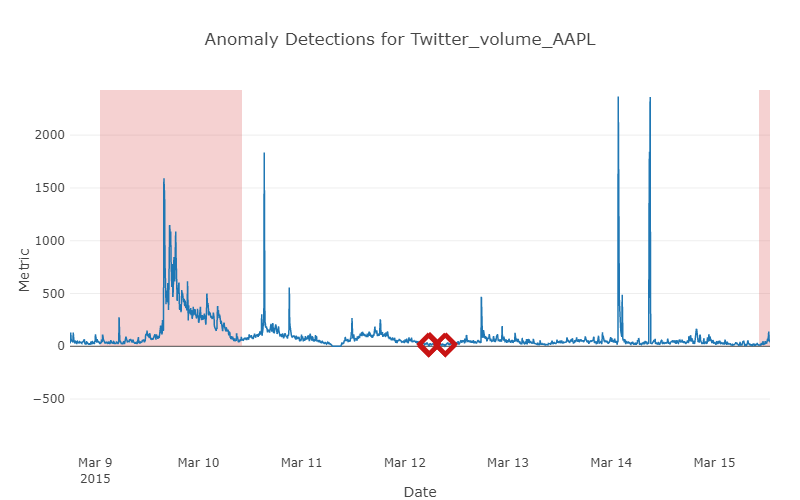
\includegraphics[width=.7\textwidth]{evaluation/lof/unreasonable_detection3.png}
        \subcaption{Another example of an unreasonable detection by \gls{lof}.}
    \end{subfigure}
    \caption[(Seemingly) unreasonable detections from \gls{lof}.]{(Seemingly) unreasonable detections from \gls{lof}. Detections are
    depicted as colored diamond symbols. Illustration by the author.}\label{fig:lof-output}
\end{figure}

\begin{figure}[htp!]
    \begin{subfigure}[b]{\linewidth}
        \centering
        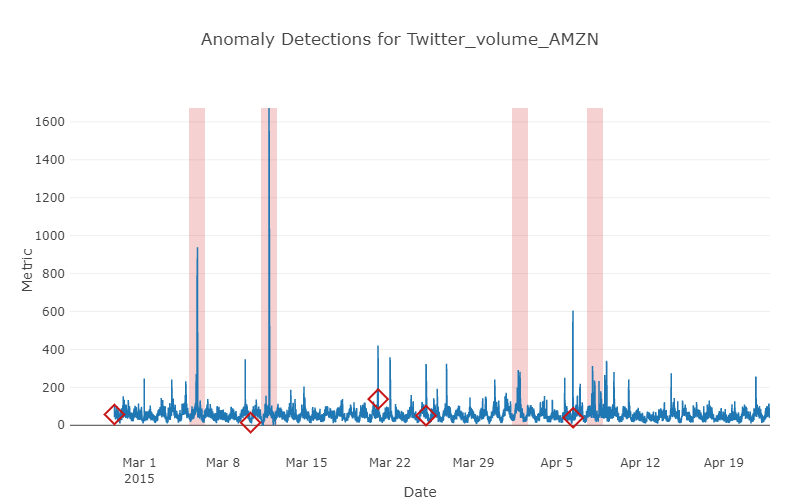
\includegraphics[width=.7\textwidth]{evaluation/dagmm/no_tp.png}
        \subcaption{False positives from \gls{dagmm}}
    \end{subfigure}%
    \\
    \begin{subfigure}[b]{\linewidth}
        \centering
        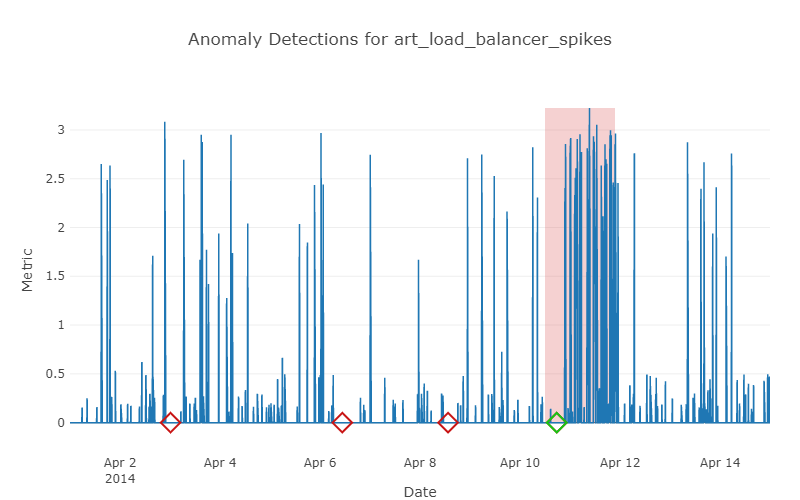
\includegraphics[width=.7\textwidth]{evaluation/dagmm/lucky_detections.png}
        \subcaption{A representative true positive from \gls{dagmm}. The
        reason for the anomaly is the high value spike (inside the red area).
        \gls{dagmm} (unreasonably) attributes the anomaly to a normal value
        approximately two days before.}
    \end{subfigure}
    \caption[Examples from \gls{dagmm}.]{Examples from \gls{dagmm}. Illustrations by the author.}\label{fig:dagmm-output}
\end{figure}

\begin{figure}[htp!]
    \begin{subfigure}[b]{\linewidth}
        \centering
        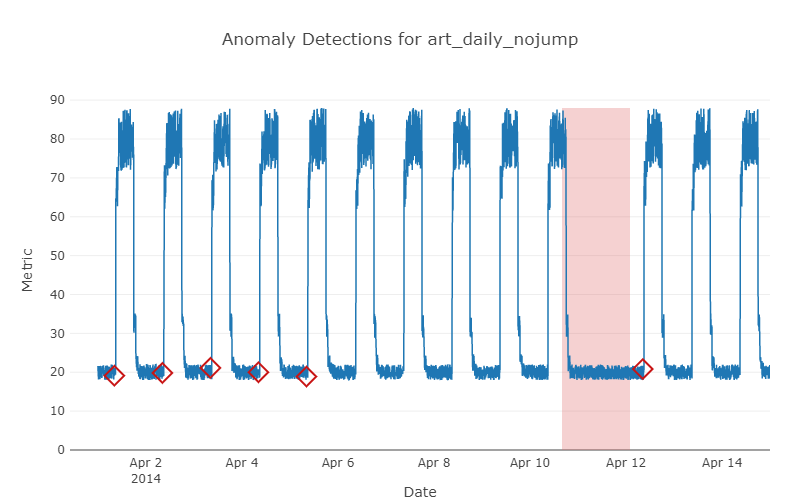
\includegraphics[width=.7\textwidth]{evaluation/rrcf/season3.png}
        \subcaption{Example detection of a cyclicity violation. Note that
        the anomaly was only detected as values began rising again for the normal
        pattern.}
    \end{subfigure}%
    \\
    \begin{subfigure}[b]{\linewidth}
        \centering
        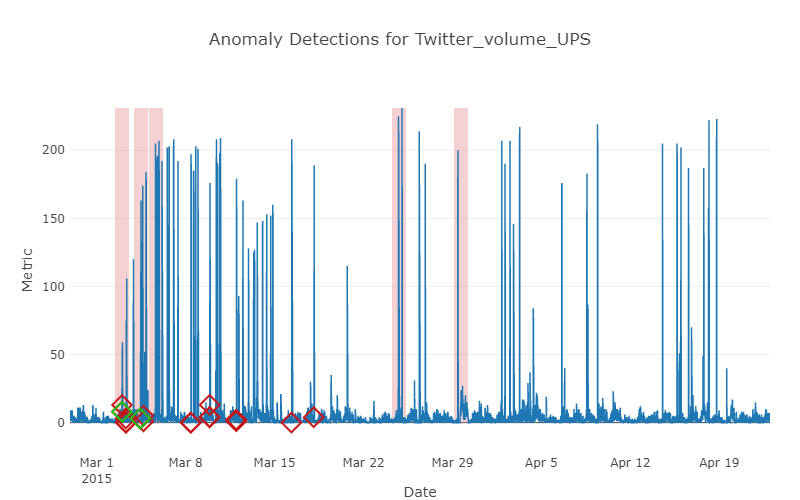
\includegraphics[width=.7\textwidth]{evaluation/rrcf/confused3.png}
        \subcaption{A representative result from \gls{rrcf}, where a complex
        time series confuses the algorithm.}
    \end{subfigure}
    \caption[Examples from \gls{rrcf}.]{Examples from \gls{rrcf}. Illustrations by the author.}\label{fig:rrcf-output}
\end{figure}

\begin{figure}[htp!]
    \begin{subfigure}[b]{\linewidth}
        \centering
        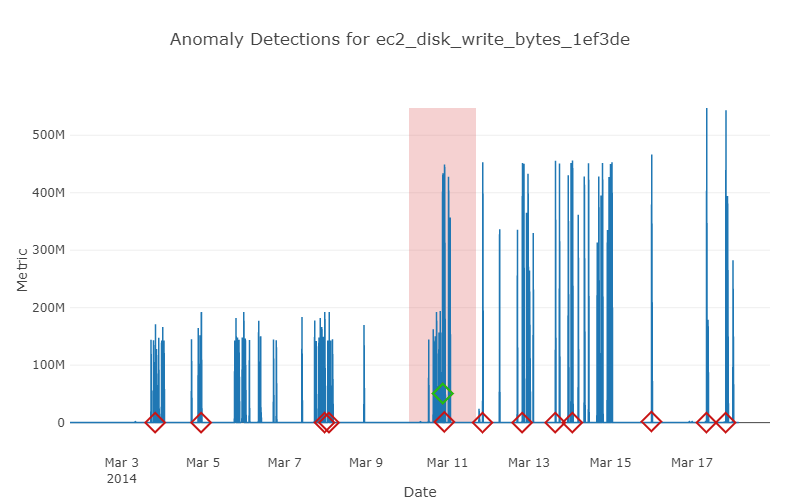
\includegraphics[width=.7\textwidth]{evaluation/khundman/highfp.png}
        \subcaption{High false positives rate on time series with many spikes.}\label{fig:khundman-fp}
    \end{subfigure}%
    \\
    \begin{subfigure}[b]{\linewidth}
        \centering
        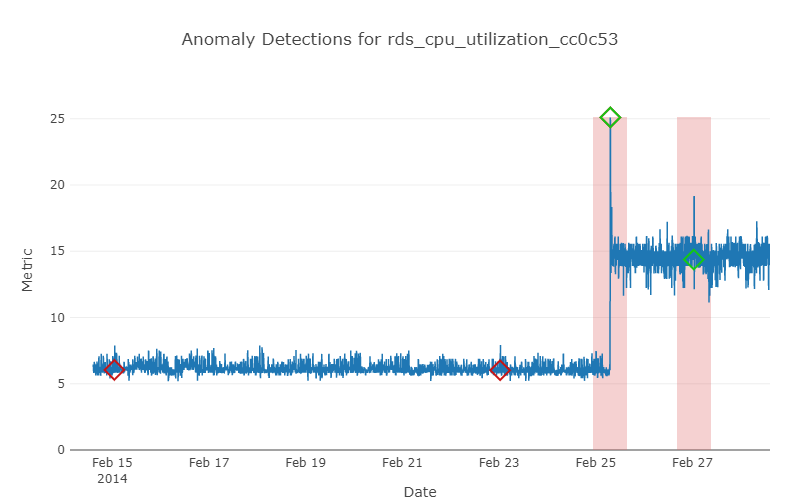
\includegraphics[width=.7\textwidth]{evaluation/khundman/success.png}
        \subcaption{Successful detection of two spikes.}\label{fig:khundman-success}
    \end{subfigure}
    \caption[Examples from \gls{ndt}.]{Examples from \gls{ndt}. Illustrations by the author.}\label{fig:khundman-output}
\end{figure}

\begin{figure}[htp!]
    \begin{subfigure}[b]{\linewidth}
        \centering
        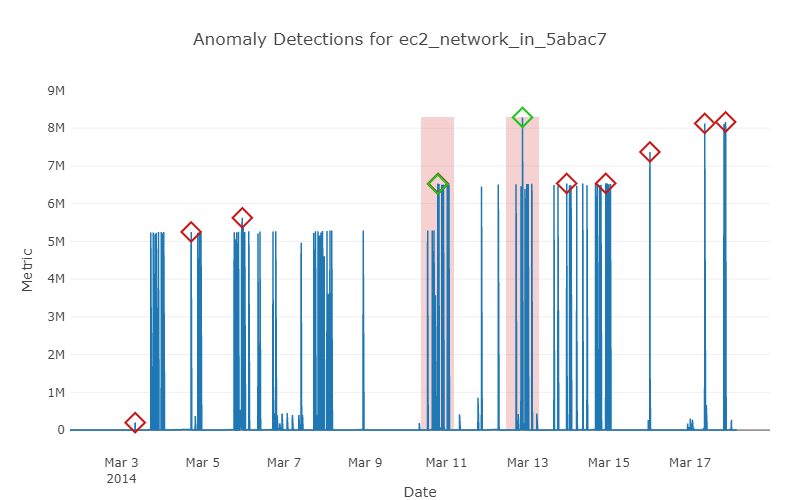
\includegraphics[width=.7\textwidth]{evaluation/lstm_ad/false-positives.png}
        \subcaption{High false positives rate on time series with many spikes.}\label{fig:lstmad-fp}
    \end{subfigure}%
    \\
    \begin{subfigure}[b]{\linewidth}
        \centering
        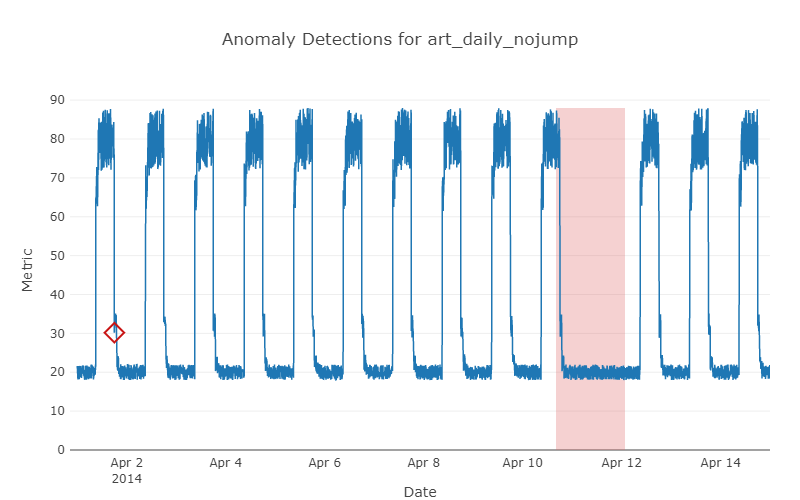
\includegraphics[width=.7\textwidth]{evaluation/lstm_ad/cyclicity.png}
        \subcaption{Cyclicity violations remain undetected by LSTM-AD.}\label{fig:lstmad-cyclicity}
    \end{subfigure}
    \caption[Examples from LSTM-AD.]{Examples from LSTM-AD\@. Illustrations by the author.}\label{fig:lstmad-output}
\end{figure}

\begin{figure}[htp!]
    \begin{subfigure}[b]{\linewidth}
        \centering
        \includegraphics[width=.7\textwidth]{evaluation/cblof/highfp.png}
        \subcaption{High false positives rate on (some) time series with irregular spikes.}\label{fig:cblof-fp}
    \end{subfigure}%
    \\
    \begin{subfigure}[b]{\linewidth}
        \centering
        \includegraphics[width=.7\textwidth]{evaluation/cblof/infreq_spikes.png}
        \subcaption{Adaptation to more regularly spiking time series.}\label{fig:cblof-cyclicity}
    \end{subfigure}
\end{figure}

\begin{figure}[htp!]
    \ContinuedFloat{}
    \begin{subfigure}[b]{\linewidth}
        \centering
        \includegraphics[width=.7\textwidth]{evaluation/cblof/good_result.png}
        \subcaption{Example of a good result from \gls{cblof}.}\label{fig:cblof-good}
    \end{subfigure}
\caption[Examples from \gls{cblof}.]{Examples from \gls{cblof}. Illustrations by the author.}\label{fig:cblof-output}
\end{figure}


\begin{figure}[htp!]
    \begin{subfigure}[b]{\linewidth}
        \centering
        \includegraphics[width=.7\textwidth]{evaluation/lstm_ed/highfp.png}
        \subcaption{High false positives rate on (some) time series with irregular spikes.}\label{fig:lstmed-fp}
    \end{subfigure}%
    \\
    \begin{subfigure}[b]{\linewidth}
        \centering
        \includegraphics[width=.7\textwidth]{evaluation/lstm_ed/harder_box.png}
        \subcaption{A harder anomaly (dotted box) detected by LSTM-ED.}\label{fig:lstmed-harder}
    \end{subfigure}
    \\
    \begin{subfigure}[b]{\linewidth}
        \begin{subfigure}[b]{.45\linewidth}
            \centering
            \includegraphics[width=\textwidth]{evaluation/lstm_ed/artificial_lstm.png}
        \end{subfigure}
        \hfill
        \begin{subfigure}[b]{.45\linewidth}
            \centering
            \includegraphics[width=\textwidth]{evaluation/lstm_ed/artificial_cblof.png}
        \end{subfigure}
        \subcaption{Left: Results from LSTM-ED on one of the artificial time series (straight line).
        Right: Results from \gls{cblof} on the same artificial time series.}\label{fig:lstmed-artificial}
    \end{subfigure}
\caption[Examples from LSTM-ED.]{Examples from LSTM-ED\@. Illustrations by the author.}\label{fig:lstmed-output}
\end{figure}

\begin{figure}[htp!]
    \begin{subfigure}[b]{\linewidth}
        \centering
        \includegraphics[width=.7\textwidth]{evaluation/knn/no_spikes.png}
        \subcaption{Two simple spike anomalies missed by \gls{knn}.}\label{fig:spike-missed}
    \end{subfigure}
    \\
    \begin{subfigure}[b]{\linewidth}
        \centering
        \includegraphics[width=.7\textwidth]{evaluation/knn/cyclicity.png}
        \subcaption{A simple cyclicity violation that was detected by \gls{knn},
        presumably due to its unusual value range.}\label{fig:knn-cyclicity}
    \end{subfigure}%
    \\
    \begin{subfigure}[b]{\linewidth}
        \centering
        \includegraphics[width=.7\textwidth]{evaluation/knn/good.png}
        \subcaption{A difficult anomaly detected by \gls{knn} (rightmost anomaly).}\label{fig:knn-harder}
    \end{subfigure}
\caption[Examples from \gls{knn}.]{Examples from \gls{knn}. Illustrations by the author.}\label{fig:knn-output}
\end{figure}


\begin{figure}[htp!]
    \begin{subfigure}[b]{\linewidth}
        \centering
        \includegraphics[width=.7\textwidth]{evaluation/threshold/good.png}
    \end{subfigure}%
    \\
    \begin{subfigure}[b]{\linewidth}
        \centering
        \includegraphics[width=.7\textwidth]{evaluation/threshold/representative.png}
    \end{subfigure}
\caption[Examples from Numenta Threshold Detector.]{Two representative examples
from the Numenta Threshold Detector. Illustrations by the author.}\label{fig:threshold-output}
\end{figure}

\begin{figure}[htp!]
    \begin{subfigure}[b]{\linewidth}
        \centering
        \includegraphics[width=.7\textwidth]{evaluation/skyline/cyclicity.png}
        \subcaption{Skyline was unable to detect cyclicity violations.}\label{fig:skyline-cyclicity}
    \end{subfigure}%
    \\
    \begin{subfigure}[b]{\linewidth}
        \centering
        \includegraphics[width=.7\textwidth]{evaluation/skyline/uncommon_spikes.png}
        \subcaption{An example of spikes that are outside the moving 3-Sigma
        rule and thereby lead to many false positives.}\label{fig:skyline-fp}
    \end{subfigure}
\caption[Examples from Skyline.]{Examples from Skyline. Illustrations by the author.}\label{fig:skyline-output}
\end{figure}

\begin{figure}[htp!]
    \begin{subfigure}[b]{\linewidth}
        \begin{subfigure}[b]{.45\linewidth}
            \centering
            \includegraphics[width=\textwidth]{evaluation/ae/ae3.png}
        \end{subfigure}
        \hfill
        \begin{subfigure}[b]{.45\linewidth}
            \centering
            \includegraphics[width=\textwidth]{evaluation/ae/lstm3.png}
        \end{subfigure}
        \subcaption{\gls{ae} (left) is able to produce one more true positive than LSTM-ED (right)
        on this example}\label{fig:lstm-vs-ae1}
    \end{subfigure}
    \\
    \begin{subfigure}[b]{\linewidth}
        \begin{subfigure}[b]{.45\linewidth}
            \centering
            \includegraphics[width=\textwidth]{evaluation/ae/result_from_ae_1.png}
        \end{subfigure}
        \hfill
        \begin{subfigure}[b]{.45\linewidth}
            \centering
            \includegraphics[width=\textwidth]{evaluation/ae/result_from_lstmed_1.png}
        \end{subfigure}
        \subcaption{\gls{ae} (left) produces one more true positive and five less false
        positives than LSTM-ED (right) on this example.}\label{fig:lstm-vs-ae2}
    \end{subfigure}
\caption[Comparison of \gls{ae} and LSTM-ED on two time series.]{Comparison of \gls{ae} and LSTM-ED on two time series. Illustrations by the author.}\label{fig:lstm-vs-ae}
\end{figure}

\begin{figure}[htp!]
    \begin{subfigure}[b]{\linewidth}
        \centering
        \includegraphics[width=.7\textwidth]{evaluation/htm/cyclicity_1.png}
        \subcaption{\gls{htm} was able to detect simple cyclicity violations in the
        artificial time (and thereby simple) series.}\label{fig:htm-cyclicity}
    \end{subfigure}%
    \\
    \begin{subfigure}[b]{\linewidth}
        \centering
        \includegraphics[width=.7\textwidth]{evaluation/htm/cyclicity_2.png}
        \subcaption{More difficult cyclicity violations were not detected.}\label{fig:htm-cyclicity2}
    \end{subfigure}%
    \\
    \begin{subfigure}[b]{\linewidth}
        \centering
        \includegraphics[width=.7\textwidth]{evaluation/htm/subtle_box.png}
        \subcaption{\gls{htm} was more sensitive for some subtle anomalies.}\label{fig:htm-subtle}
    \end{subfigure}
\end{figure}

\begin{figure}
    \ContinuedFloat{}
    \begin{subfigure}[b]{\linewidth}
        \centering
        \includegraphics[width=.7\textwidth]{evaluation/htm/unreliable_on_fast_fluctuation.png}
        \subcaption{\ldots while other subtle anomalies were overlooked.}\label{fig:htm-subtle-overlooked}
    \end{subfigure}
    \\
    \begin{subfigure}[b]{\linewidth}
        \centering
        \includegraphics[width=.7\textwidth]{evaluation/htm/high_fp_regular_high_spikes.png}
        \subcaption{\gls{htm} did not adapt to regular yet infrequent value spikes.}\label{fig:htm-spikes}
    \end{subfigure}
\caption[Examples from \gls{htm}.]{Examples from \gls{htm}. Illustrations by the author.}\label{fig:htm-output}
\end{figure}

%%%% General Todos: %%%%

\end{document}